{\setstretch{1.0} \textit{Manuscript in preparation.} \par}%Paper reference, note, other. Can remove. Single line space.
\section*{Abstract}
{\setstretch{1.0}  
Type 1 diabetes is a systemic disease triggered by a local autoimmune inflammatory reaction in the insulin-producing cells. The disruption of the glucose-insulin-glucagon system induces organ-wide, long-term effects on glycolytic and non-glycolytic processes. Mathematical modeling of the whole-body regulatory bihormonal system helped identifying intervention points to ensure a better control of type 1 diabetes mellitus. We present a whole-body model, developed using an integrative modeling framework termed CRONICS, linking regulation and metabolism in an organ-resolved manner. The developed framework allowed to correctly predict disrupted metabolic processes in type 1 diabetes in relation to the symptoms, highlighted common pathophysiological processes with neurodegenerative disorders and suggested calcium channel blockers as potential adjuvants for diabetes control. Additionally, the model predicted an insulin-dependent rewiring of inter-organ crosstalk. Moreover, it allowed to assess the impact of inter- and intra-individual variability to insulin treatment and their implications on clinical outcome. In particular, GLUT-4 is suggested as a potential pharmacogenomics regulator of intra-individual insulin efficacy. The organ-resolved, dynamic model opens the way to better understand human pathology and the model-based design of precise allopathic strategies.
\par}%single line space

\newpage
\begin{figure}[!htp]
\centering
	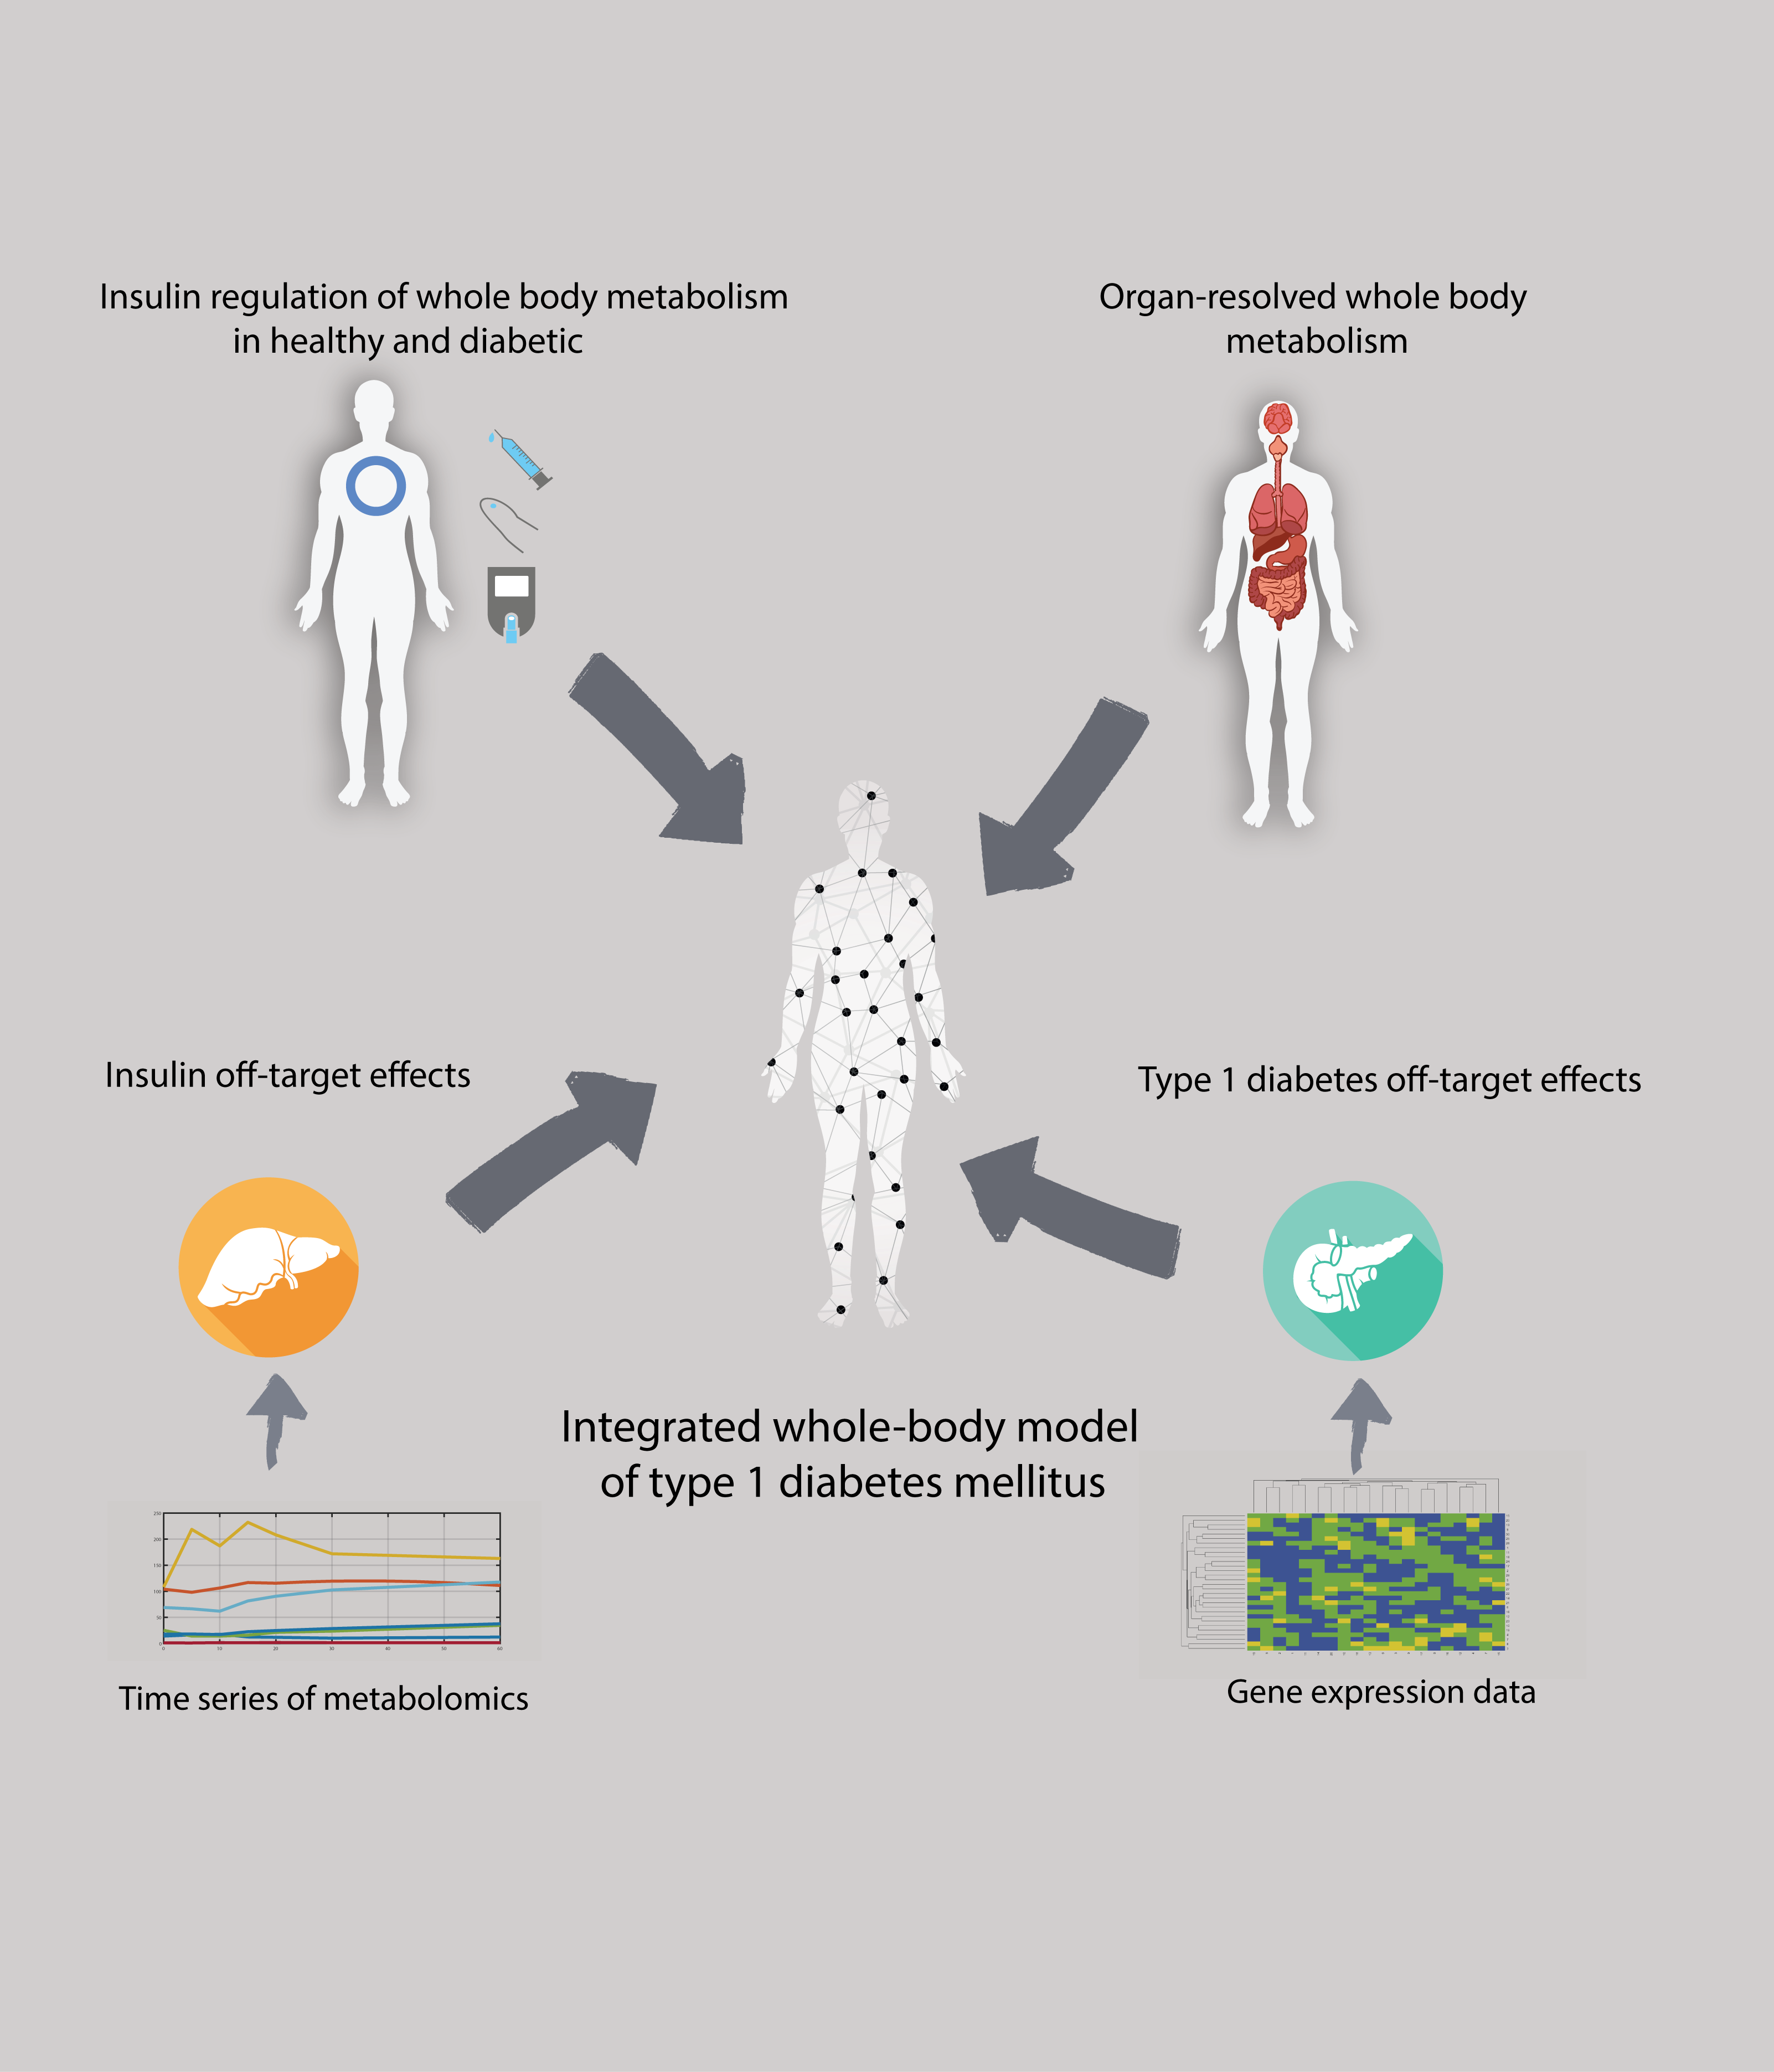
\includegraphics[width=\textwidth,height=\textheight,keepaspectratio]{GIM/studySummary.png}%Figure from images\Figure1.png
	\caption[Study summary of whole-body dynamic metabolism.]{Study summary of whole-body dynamic metabolism in type 1 diabetes. A whole-body dynamic model of type 1 diabetes integrates a whole-body, organ-resolved metabolic model (Harvey), with a whole-body dynamic model of the glucose-insulin-glucagon system (GIM), type 1 diabetes gene expression in the pancreas, and insulin-induced metabolite concentration time-course. The model captured the state-of-the-art knowledge about type 1 diabetes and gave insights into within and between-patient variability to insulin response.}
	\label{fig:GIMSummary}
\end{figure}

\newpage
\section{Introduction}
Type 1 diabetes (T1D) mellitus is a systemic disease triggered by the destruction of insulin-producing pancreatic beta cells \cite{maahs2010epidemiology}. The World Health Organization estimated the incidence of up to 36.8 new cases in 100,000 persons per year with an increase of 2 to 5\% worldwide \cite{maahs2010epidemiology}. It remains the most prevalent type of diabetes in children and has cumbersome lifelong effects \cite{maahs2010epidemiology}. The disease affects primarily the production of insulin causing acute metabolic complications and coronary artery disease, resulting in high early mortality rates \cite{orchard2006type}. Additionally, the misdiagnosis of T1D in adults is a recently acknowledged issue \cite{thomas2017frequency}, as the delay in implementing the insulinotherapy can further exacerbate the disease symptoms.
The systemic mechanism of action of insulin induces the whole-body semiology of T1D. The symptoms include several glucose dependent metabolic processes such as micro- and macroangiopathy, diabetic retinopathy, and nephropathy, as well as fatty acids related implications like atherosclerosis and cardiovascular disease \cite{american2014diagnosis}. Supplementing patients with exogenous insulin remains the gold standard treatment of type 1 diabetes. Although being  very efficient in preventing biochemical alterations, insulin has a high within and between subject variability that can induce adverse reactions ranging from hypoglycemia to uncontrolled diabetes; effects that can hamper the treatment compliance \cite{heinemann2002variability}.\\
The wealth of data in type 1 diabetes helped the development of whole-body mathematical models of insulin action and disease progression, notably the ODE-based glucose insulin model (GIM) \cite{schaller2013generic}. GIM includes fine-grained details of tissue-based insulin and glucagon action in relation to glucose dynamics such as insulin-dependent receptor synthesis and the gastrointestinal hormonal regulation of glucose levels. It could also reproduce the outcome of differential diagnosis tolerance tests on type 1 diabetic patients. The model extensively described the bihormonal regulatory events yet modeling of metabolism remained limited to the first step of glycolytic pathways.\\
Therefore, the systematic analysis of disrupted metabolic processes beyond glycolysis in type 1 diabetes needs extended approaches. To better capture metabolism, we used the constraint-based reconstruction of the organ-resolved whole-body human metabolic network (Harvey) \cite{thiele2018metabolism}. Harvey includes the tissue-specific metabolic pathways of 20 organs, six sex organs, and six blood cells enabling thereby the modelling of carbohydrate disorders and the study of their impact on non-glycolytic pathways. Therefore, the whole-body model provides a complete picture of organ-resolved human metabolism, yet addressing disease dynamics and the patient's response to insulin requires the modeling of both the metabolic pathways as well as non-metabolic processes including insulin receptor binding, transduction of signal, and internalisation of receptors. Recently, multi-scale, multi-algorithm, whole-organism dynamic models in biology \cite{oyaas2017genome} have seen a surge in complexity, addressing mostly microbiology \cite{karr2012whole,covert2008integrating}, plant physiology \cite{grafahrend2013multiscale}, and also human physiology and xenobiotic metabolism \cite{krauss2012integrating}. 
Accordingly, we coupled the organ-resolved whole-body model (Harvey) with the dynamic glucose insulin ODE-based model (GIM). The multiscale model (dHarvey) allowed to represent type 1 diabetes through both glycolytic target effects and off-target effects that were mapped onto the model using gene expression data. Particularly, the effects of insulin were added through including an additional dynamical model representing its impact on liver metabolism. The model including the target and off-target effects of both type 1 diabetes and insulin, allowed to i) quantify disrupted metabolic process in type 1 diabetes in relation the disease symptomatology, ii) assess insulin non-glycolytic effects, and iii) shed new light on mechanisms underlying inter and intra-individual variability of insulin effects. The hybrid model provides a kernel for the organ-specific integration of biological data and paves the way for predictive human physiology.

\section{Methods}
\subsection{Coupling the dynamical model and the constraint-based model} \label{meth1}
Determining the metabolic reaction flux in the constraint-based model (Harvey) requires solving the usual liner program:
\begin{alignat*}{2}
  & \text{max: } &  & c^{T}v_{H}\\
  & \text{subject to: } &  &  
                \begin{aligned}[t] \\
                & Sv_{H} = b_{H} \\
                & v_{min} \leq v_{H}  \leq  v_{max}
                \end{aligned}
\end{alignat*}
,with $c$ the objective coefficient vector, $S_{m,n}$ the stoichiometric matrix of $m$ metabolites and $n$ reactions, $v_{H}$ the flux vector bounded by $v_{min}$ the lower bound vector and $v_{max}$ the upper bound  vector. When $b_{H}=0_{m}$, the problem is constrained by $Sv=0$, also referred to as Flux Balance Analysis (FBA) \cite{orth2010flux}.\\
Points of intersection between the dynamical model (GIM) and the constraint-based model (Harvey) included metabolites and reactions. There were four classes of correspondences (Figure \ref{fig:GIM0}) that resulted in different implementations of the coupling constraints (Text \ref{GIM:sp1}). Let us first consider the concentrations of a given metabolite modelled in GIM (G) by the following ODE:
\begin{equation*}
\frac{dC_{G,n}}{dt}=X_{G,prod}-X_{G,elim}
\end{equation*}
,with $X_{prod}$ and $X_{elim}$ are reaction fluxes respectively producing and eliminating the metabolite $n$ through first order processes.\\
Case 1: If one reaction in the dynamical model corresponded to one reaction in the metabolic model, the constraints for one time step were subjected as follows:
\begin{equation*}
v_{H,i}=X_{G,j}
\end{equation*}
,with $t$ as the time, $v$ the flux vector, $i$ the index of the reaction in the Harvey model ($H$), and $j$ the index of the reaction in the GIM model such that reactions $i$ and $j$ perform the same metabolic function, e.g., liver hexokinase reaction.\\ 
Case 2: When a metabolite is represented in both models, the sum of its anabolic and catabolic fluxes in Harvey is constrained by its change-of-concentration in GIM, also referred to as metabolite pooling fluxes \cite{covert2008integrating}. The constraints are formulated as the following:
\begin{equation*}
b_{H,m}=\frac{dC_{G,n}}{dt}
\end{equation*}
,with $m$ referring to the metabolite in Harvey, $n$ the metabolite in GIM, $C_n$ the concentration of $n$, and $b$ the vector of metabolite change-of-concentration in Harvey. \\
Case 3: The third case corresponds to one reaction in GIM being represented by more than one reaction in Harvey. Typically, they correspond to reactions catalyzed by cofactor-dependent enzymes such as hexokinase with ATP and ADP as cofactors. The reaction pooling fluxes are then subjected as follows:
\begin{equation*}
\sum_{i=1}^{k} v_{H,i}=X_{G,l}
\end{equation*}
,with $v_1$ to $v_k$ are the reactions in Harvey corresponding to reaction $l$ in GIM. \\
Case 4: In the case when one metabolite in GIM corresponds to more than one metabolite in Harvey, such as blood cells glucose in GIM corresponding to glucose in red blood cells, monocytes, natural killer cells, B cells, platelets, and CD4 T cells in the metabolic model, the constraints are formulated as follows:
\begin{equation*}
\sum_{i} (v_{H,a(i)}+v_{H,c(i)})=\frac{dC_{G,j}}{dt}
\end{equation*}
,with $v_a$ the anabolic fluxes, $v_c$ the catabolic fluxes, $i$ the index of the different metabolites in Harvey corresponding to metabolite $j$ in GIM. 
After subjecting the constraints, the steady-state was assumed in the chosen time step for the non-overlapping metabolites in both models, such as amino acids. The constraints then translates to the following:
\begin{equation*}
S.v_{H}=b_{H}
\end{equation*}
,with $S$ the stoichiometric matrix of Harvey, $v$ the flux vector, and $b$ the metabolite concentration change, that equalled zero for steady-state metabolite and non-zero for metabolites falling under case 2. When the applied constraints rendered the linear program infeasible, the lower and upper bounds were relaxed minimally in both the amplitude of relaxation and the cardinal of the reactions to be relaxed (Text \ref{GIM:sp2}).\\
The simulation of tolerance tests, and the assessment of the inter and intra-individual variability to insulin response were performed using dHarvey with specific model parameters. The tolerance tests parameters were as reported in the GIM model \cite{schaller2013generic} (Table \ref{GIM:tbls3}), which includes trials in healthy and T1D patients for intravenous insulin tolerance test (IVITT), intravenous glucose tolerance test (IVGTT), baseline glucose concentration (Noinf), subcutaneous insulin bolus (SCIB), subcutaneous insulin infusion (SCII), solid meal (WB-Solid), oral liquid glucose solution (WB-Liquid). The parameters of the GIM model were reportedly \cite{schaller2013generic} identified using tolerance tests trial data \cite{sorensen1985physiologic,regittnig1999plasma} and bihormonal closed-loop experiments \cite{el2010bihormonal}. Harvey was simulated using exchange reactions corresponding to standard European diet \cite{sahoo2013predicting}.
\subsection{Comparison of the predictive capabilities of the different models}
In order to compare the predictive capabilities of Harvey, GIM, and dHarvey, we simulated the intravenous glucose tolerance test (IVGTT). GIM includes a parameter set for simulating IVGTT (Table \ref{GIM:tbls3}) and glucose concentrations were obtained through integrating the ODEs.\\
Glucose concentrations in Harvey alone were obtained through dFBA. Briefly, the initial amount of glucose is set as availability constraints and decreases in every time step after subtracting the consumed glucose fluxes obtained through solving the linear program \cite{mahadevan2002dynamic}. The maximum rate-of-change of glucose was set to the intravenously injected amount in the $b$ vector, the problem translates then to the following:
\begin{alignat*}{2}
  & \text{max: } &  & c^{T}v\\
  & \text{subject to: } &  &  
                \begin{aligned}[t] \\
                & Sv \leq b \\
                & v_{min} \leq v  \leq  v_{max}
                \end{aligned}
\end{alignat*}
dHarvey not only reproduced the glucose time series of GIM but also could predict the time course of ATP, which is not present in GIM. The simulation was done through setting ATP demand reaction in each time step as the objective function as the following:
\begin{alignat*}{2}
  & \text{max: } &  & c^{T}v\\
  & \text{subject to: } &  &  
                \begin{aligned}[t] \\
                & Sv=0 \\
                & v_{min} \leq v  \leq  v_{max}
                \end{aligned}
\end{alignat*}
, with $c$ the vector of objective function coefficients and $v_{min}$,$v_{max}$ respectively, the minimum and maximum flux going through the reaction. The $c$ vector entry corresponding to the indices of reactions corresponding to ATP demand in every organ were set to one. Then, the baseline value of ATP demand reaction flux, calculated at the initial simulation time, was subtracted from the obtained value. A cumulative sum of the resulting fluxes allowed to get the theoretical time course of ATP in a given tissue. 
\subsection{Modeling T1D off-target effects in the pancreas}
We considered T1D as the combination of target and off-target effects. The target effects are directly related to the decrease of insulin secretion and the increase of glucose levels and the off-target effects are represented in the underlying chronic inflammation that triggers the disease. To model target effects, we constructed dHarvey healthy and T1D models that were obtained through coupling Harvey with healthy and T1D GIM models. Moreover, consensus gene expression data \cite{planas2010gene} of pancreas biopsies of type 1 diabetic patients obtained through whole genome sequencing of four patients after five days, nine months, five years, and ten years post-diagnosis were used to further constrain the dHarvey diabetic model and to capture the chronic inflammation in the pancreas leading to the development of T1D. Differentially expressed genes were mapped on the metabolic model in order to represent the off-target effects of the disease. Among the list of 475 differentially expressed genes, only the metabolic genes present in Harvey were kept for further analysis, corresponding to 24 genes (Table \ref{GIM:tbls1}). 
Consequently the bounds in the linear program of dHarvey T1D model, were modified in the reactions corresponding to every gene such that:
\begin{gather*}
v_{min(i)}^t=v_{min(i)}^h*fc \\
v_{max(i)}^t=v_{max(i)}^h*fc \\
v_{min(i)}^t<v_i^t<v_{max(i)}^t
\end{gather*}
, with $fc$ the gene expression fold change between control and disease of the gene encoding reaction $i$, $v_{min(i)}^h$  the minimum reaction flux corresponding to reaction $i$ in the healthy model, and $v_{max(i)}^h$ the maximum reaction flux of the healthy model as identified by flux variability analysis. $v_{min(i)}^t$ and $v_{max(i)}^t$ are the new lower and upper flux bound computed in dHarvey type 1 diabetic models. Gene expression allowed to constrain a total of 80 reactions in the pancreas (Table \ref{GIM:tbls2}).
\subsection{Modeling insulin off-target effects in the liver}
Similarly to T1D, we considered insulin to induce target and off-target effects. The target effects of insulin is the reduction of glucose levels, and the off-target effects are the various physiological processes involving insulin such as the regulation of glycolysis. The off-target effects of insulin in the liver were modelled through coupling an additional ODE model to the dHarvey model. The model \cite{yugi2014reconstruction} represented the metabolic effects of insulin on glycolytic fluxes during one hour. The amounts of eight metabolites \textit{in vitro} (fructose-6-phosphate, fructose-1,6-diphosphate, phosphoenolpyruvate, isocitrate, 2-oxoglutarate, malate, frucotse-2,6-biphosphate, and citrate) were scaled to amounts (mmol) \textit{in vivo} as following: 
\begin{equation*}
A_{invivo}=C_{invitro}*V_{hep}*HPGL*V_l
\end{equation*} 
,where $V_{hep}$ is the hepatocyte volume, $HPGL$ is the hepatocellularity, $C_{invitro}$ is the concentration of the metabolites \textit{in vitro} and $V_l$ the liver volume.
The values of the parameters were set as following \cite{heinemann1999standard}:
\begin{gather*}
V_{hep}=3,4.10^{-9} \quad cm^3 \\
HPGL=86.\frac{10^6 cells}{gram \, of \, liver}\\
V_l=322.6 \quad gram
\end{gather*}
The constraints were applied by setting the metabolites rate-of-change in the insulin dynamical model equal to the corresponding $b$ vector value in Harvey.
\subsection{Simulation of inter-individual variability to insulin response}
In order to assess the between subject variability of glucose dynamics after a bolus of insulin (Table \ref{GIM:tbls3}), the identified differential parameters \cite{schaller2013generic} (Table \ref{GIM:tbl1}) between type 1 diabetes and healthy GIM models were randomly varied within 2-fold interval to reproduce the observed 25-35\% of variability in a patient population \cite{heinemann2002variability} as computed by $\frac{std(AUC)}{mean(AUC)}$, where $AUC$ refers to the area under the curve of peripheral glucose concentrations per patient. The parameters were randomly increased or decreased for a synthetic group of 30 patients and the coupling between the newly obtained GIM models and Harvey was performed as described previously.  
\subsection{CRONICS, the simulation algorithm}
The simulations were done following two main methods: direct and indirect coupling \cite{covert2008integrating,krauss2012integrating}. Indirect coupling was used to dynamically constrain Harvey with respect to each time step. First, GIM is simulated for the entire time horizon and the constraints are computed and applied retrospectively to Harvey as described previously (Section \ref{meth1}, Figure \ref{fig:GIM0}). Direct coupling assumes an interdependency of both model, where the fluxes of GIM for a specific time step are passed to Harvey, and where the result of the linear program defines the initial rates in GIM for the consecutive time step. Here the outcome of the simulation of GIM is dependent on Harvey and vice-versa. The integrative framework CRONICS (Figure \ref{fig:s3GIM}) included the above mentioned coupling scenarii (Text \ref{GIM:sp3}) and additionally ensured the smoothness of the hybrid model. In fact, due to the alternate optimal solution (AOS) space , maintaining the smoothness of dynamical simulations in large-scale metabolic models could be challenging. We addressed this issue through i) performing pFBA in each time step to obtain a reduced AOS space as suggested previously, \cite{toroghi2016multi}, ii) minimizing the euclidean distance between flux vectors in each time step similarly to MOMA \cite{segre2002analysis}, and iii) optimizing for a set of reactions in each time step as suggested previously \cite{gomez2014dfbalab}. The latter was used to simulate the intra-individual variability to insulin response. Additionally, the solver parameters had to be tuned in order to optimize convergence and ensure feasibility (Text \ref{GIM:sp4}).
\subsection{Metabolic network topology}
To analyse topological features under different sets of perturbation, Harvey, which is a hypergraph of metabolism, was transformed into a metabolite-centric graph and redundant metabolite, i.e., $ATP$, $ADP$, $H_20$, $NH_4$, $H^+$, $NADH$, $NADPH$, and $Pi$ were taken out to facilitate the subsequent analysis. It was previously shown that metabolic graphs are scale-free networks, endowed with modular organization \cite{jeong2000large}. The distribution of metabolite connectivity across the metabolic network was accordingly fit on a power law as following:
\begin{equation*}
P(k)=a*k^{-\gamma}
\end{equation*}
, where $k$ represents the metabolite degree, $a$ and $\gamma$ are power law parameters, and $P(k)$ is the relative frequency of each metabolite. 
\subsection{Sensitivity analysis of the hybrid model, intra-individual variability, and multivariate regression}
In order to assess intra-individual variability to insulin injection, the GIM model parameters were fixed for the mean patient anthropomorphic parameters \cite{schaller2013generic} and the flux values of a set of 2,817 randomly selected reactions representing all the subsystems in the organs of Harvey model, were allowed to vary through assigning random objective coefficients. Consequentially, a matrix $X_{(p,q)}$ of objective coefficients for every reaction was randomly generated, with $p$ as the number of trials representing within-patient metabolic states and $q$ as the number of reactions.\\
The output of the simulation of every trial with the corresponding objective coefficients was measured in the concentration of glucose reached after insulin subcutaneous injection at each of the $n$ time step.  
The vector $Y_{(p,n)}$ is the subsequently obtained output vector containing the concentration values at each time step. Using multivariate regression, the sensitivity vector $\rho$, representing the contribution of each reaction flux in Harvey to the time-course of metabolites in GIM was computed as following:
\begin{gather*}
X* \rho \approx Y \\
\rho=(X^{T}X)^{-1}X^{T}Y
\end{gather*}
The $\rho$ vector allows then to quantify the sensitivity of peripheral glucose concentration to the considered metabolic reactions. Particularly, the minimal concentration $(C_{min})$ and in the final concentration reached at the end of the simulation $(C_{end})$ were considered for further analysis.
\begin{figure}[!htp]
\centering
	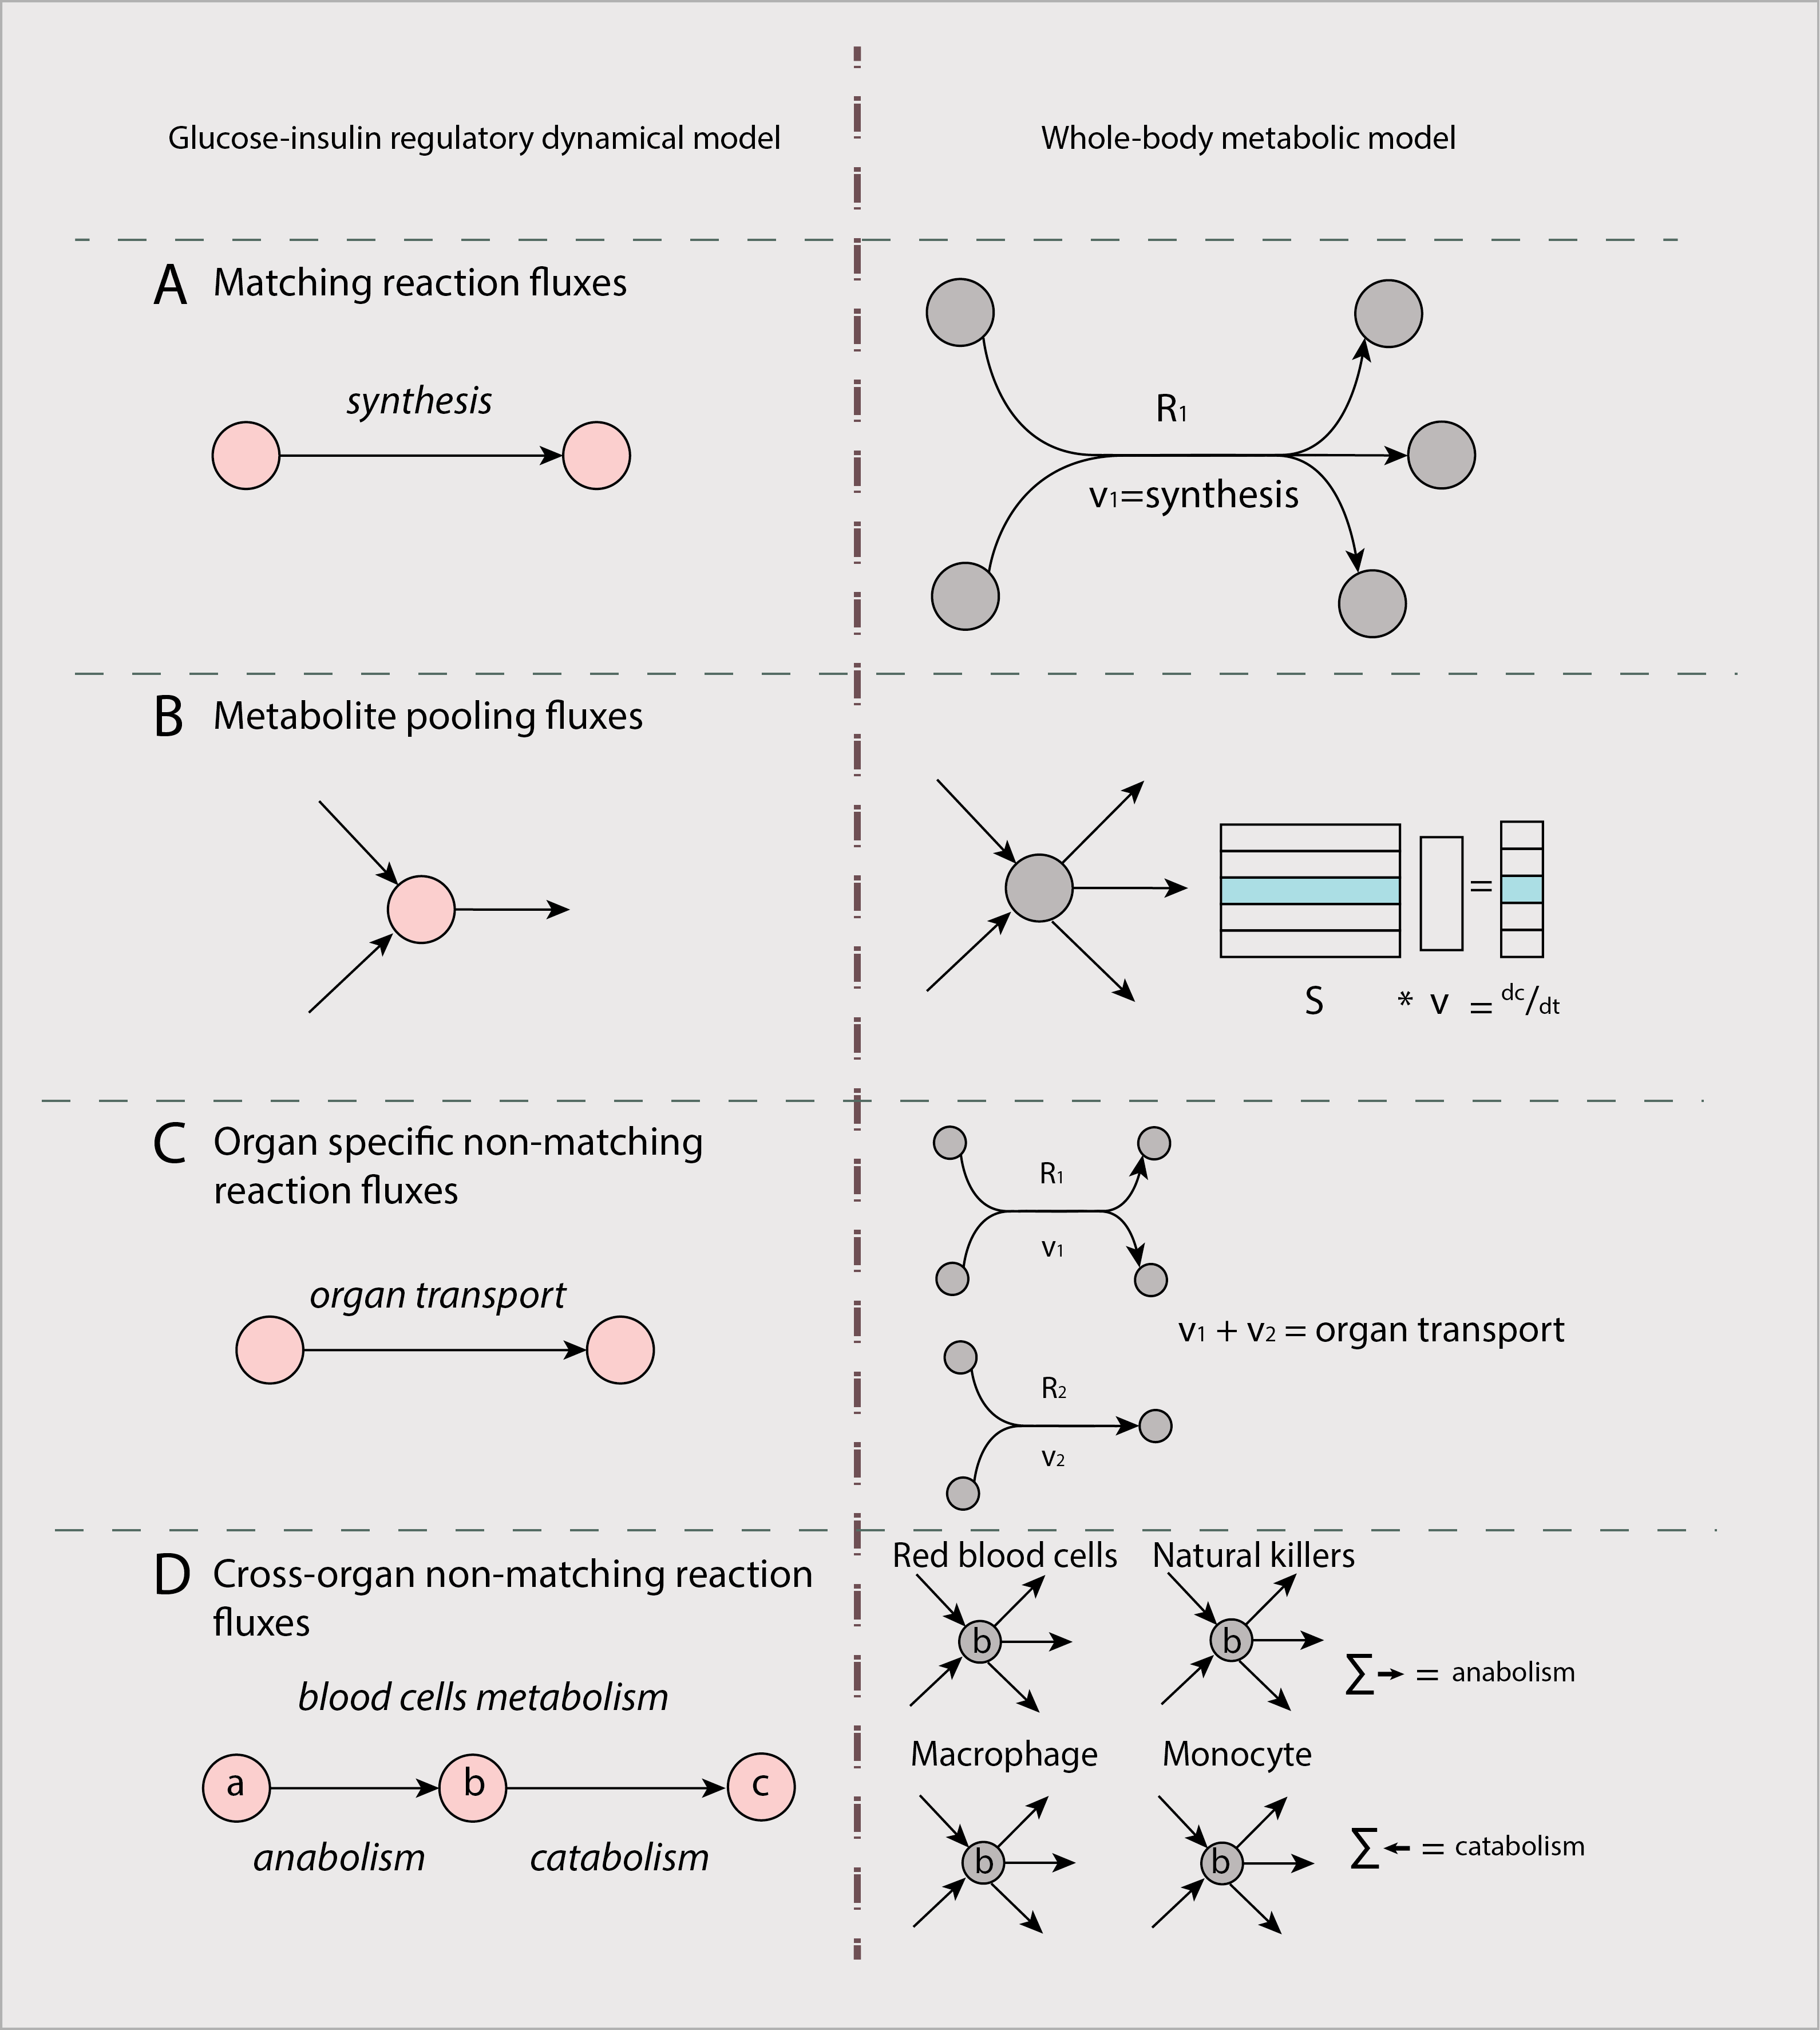
\includegraphics[width=\textwidth,height=\textheight,keepaspectratio]{GIM/figure0.png}%Figure from images\Figure1.png
	\caption[Mapping of dynamical constraints from GIM to Harvey.]{(Continued on the following page)}
	\label{fig:GIM0}
\end{figure}
\begin{figure}[t]
  \contcaption{Subjected constraints from GIM to Harvey. The constraints followed four main scenarii: A- Matching reaction flux corresponds to the case when a reaction in GIM is represented in the same way in Harvey. In this case the fluxes match fully. B-Metabolite pooling fluxes correspond to the case where the rate-of-change of a metabolite in GIM is set as a constraint in the right hand side ($b$ vector) of the linear programming problem in Harvey. C-Organ-specific non-matching reaction fluxes is the case where one reaction in GIM corresponds to more than one reaction in the same organ of Harvey. D-Cross-organ non-matching reaction fluxes. In this case, one tissue in GIM is represented by at least one compartment in Harvey. The sum of cross-organ anabolic (respectively catabolic) fluxes are set equal to the anabolic (respectively catabolic) fluxes in GIM. This case is typically related to blood cells.}% Continued caption
\end{figure}
\section{Results}
Our approach to construct a whole-body model of carbohydrate metabolism consisted of the integration of a dynamical regulatory model of a glucose insulin model (GIM) with a whole-body model of human metabolism (Harvey). The hybrid model (dHarvey) had a better predictive ability than each model on their own and showed notable differences between healthy and type 1 diabetes metabolic states. The off-target effects of both type 1 diabetes and the insulin treatment were modeled at the metabolic level using gene expression data of T1D and the metabolomics of insulin treatment. Therefore, dHarvey included the different scales of glucose metabolism (gene expression, regulation loops and metabolism). The modeling of both the target and off-target effects of T1D and insulin allowed to address the between and within-patient variability to insulin.
\begin{figure}[!htp]
\centering
	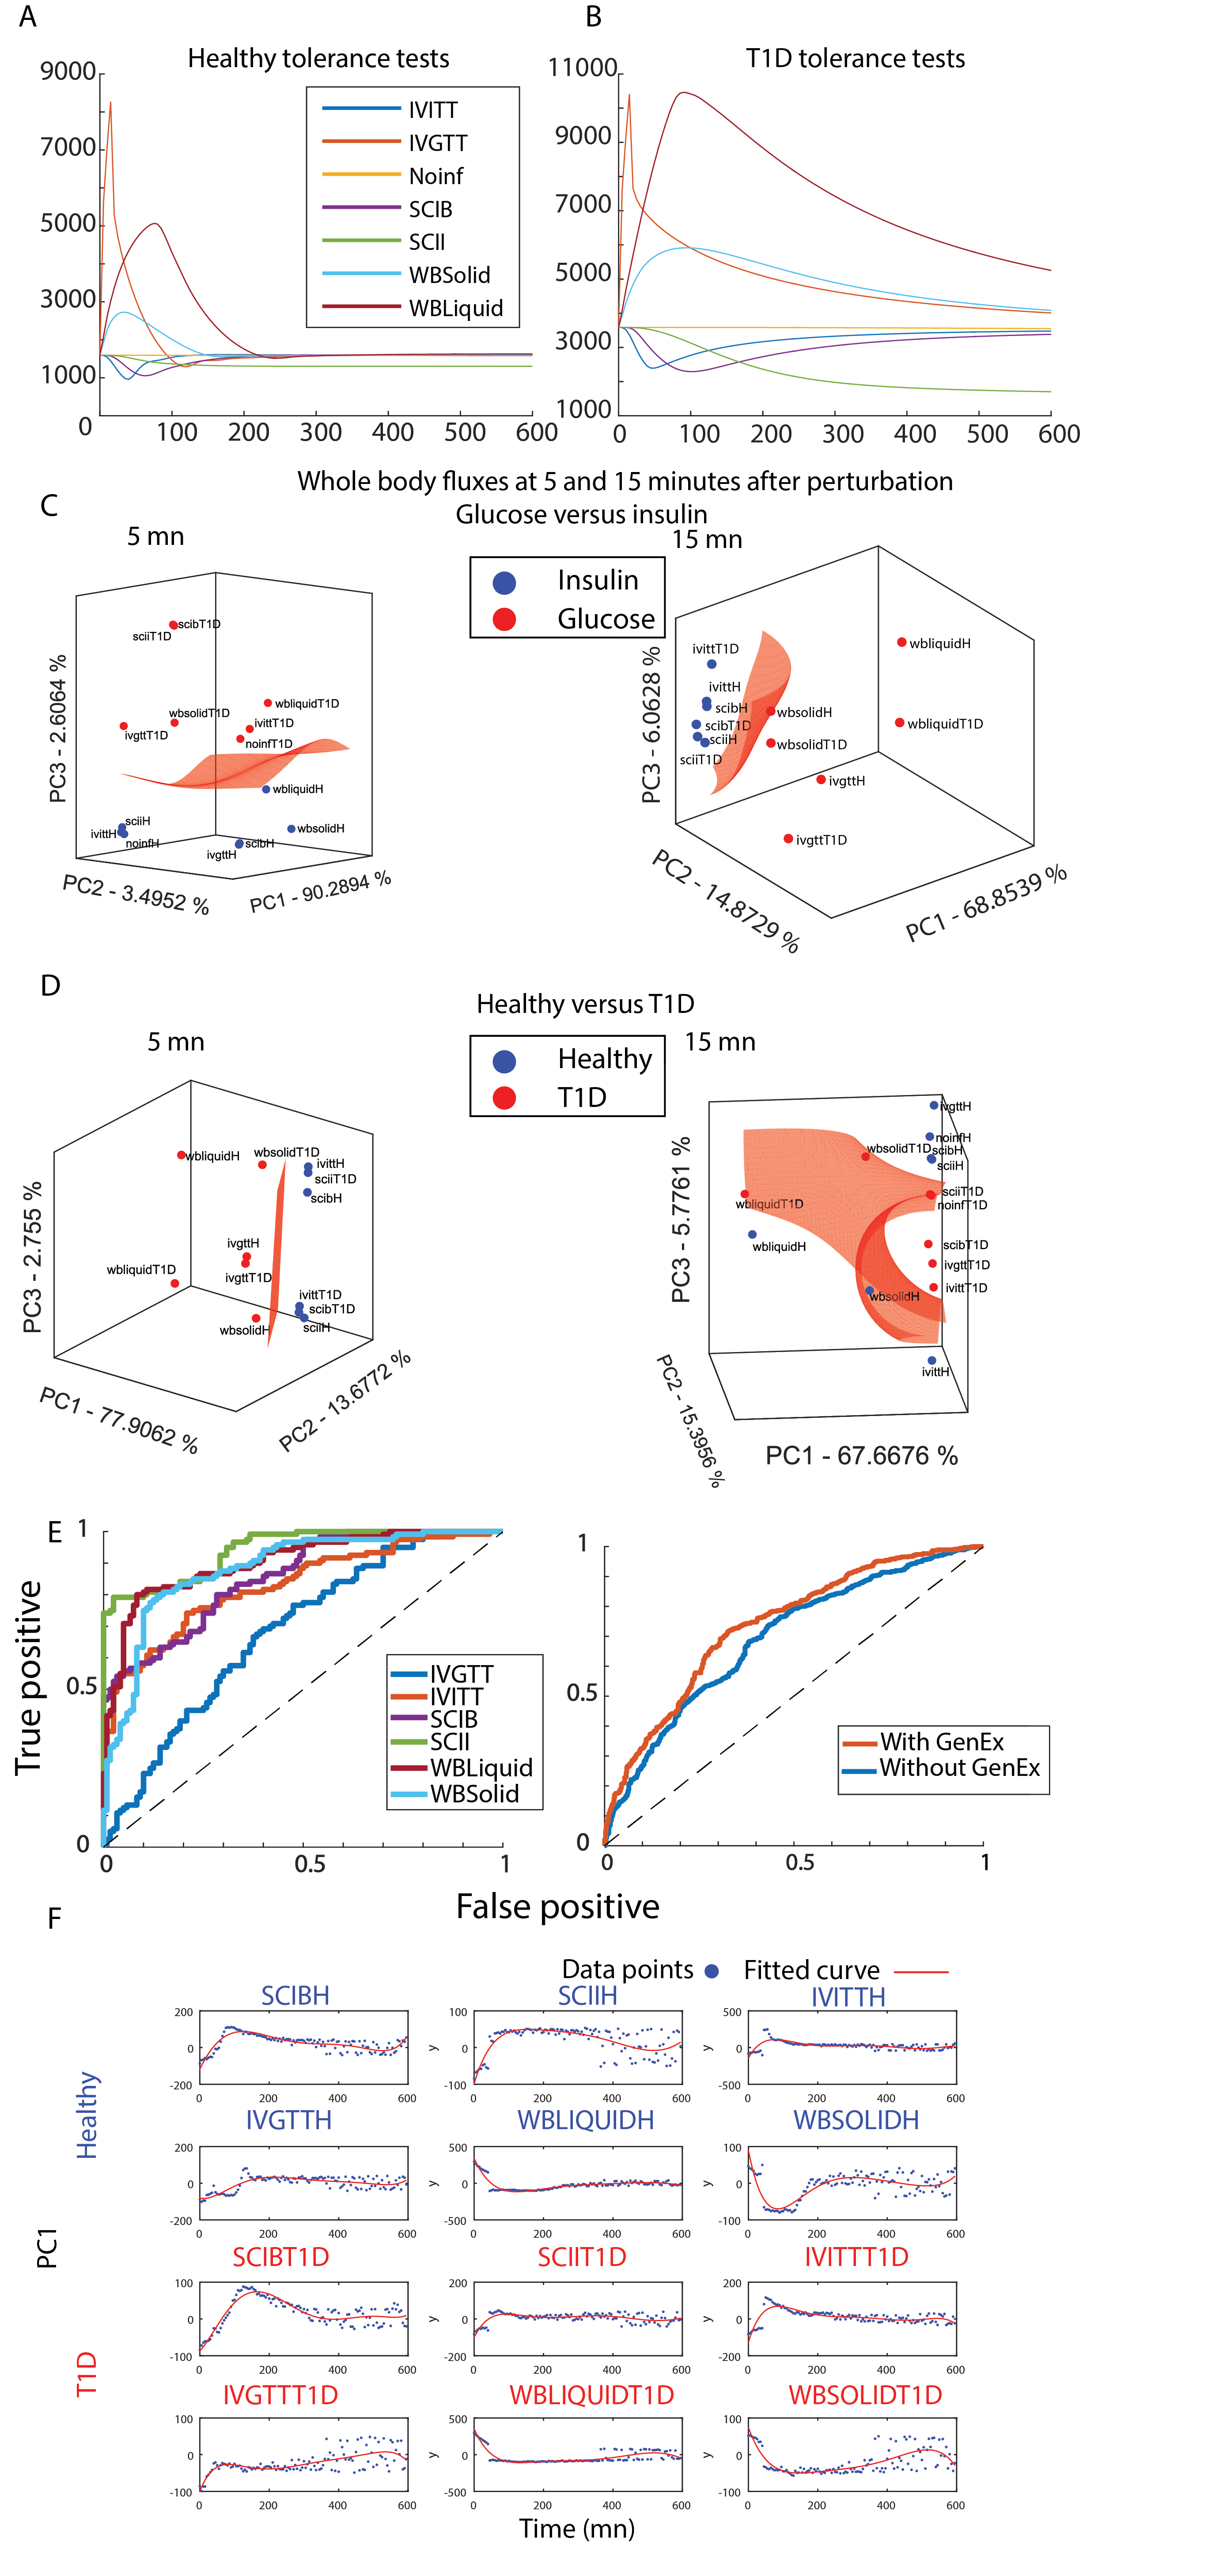
\includegraphics[width=\textwidth,height=\textheight,keepaspectratio]{GIM/figure1.png}%Figure from images\Figure1.png
	\caption[T1D induces a whole-body metabolic shift.]{(Continued on the following page)}
	\label{fig:GIM1}
\end{figure}
\begin{figure}[t]
  \contcaption{Whole-body reaction flux dynamics classify type 1 diabetes and healthy. A-Time course of glucose in peripheral blood in healthy and B-type 1 diabetes in the different tolerance tests using GIM. C-Principal component analysis of whole-body metabolic fluxes in insulin and glucose challenges and D-in healthy and T1D dHarvey models at five and 15 mn after perturbation using three first components. The support vector machine Gaussian boundary was plotted to assess the separation between classes. E-ROC curves of T1D classification. Whole-body flux dynamics over 600 minutes of simulation discriminate between healthy and T1D in each tolerance test alone (left) and in a combination of all tolerance tests in a binary classifier (right), where adding gene expression constraints showed a higher predictive capability of the model towards T1D. F-Time-course of the first principal component (PC1) of the flux vector in each time step in the different tolerance tests showed a shift in global metabolism as a result of glucose dynamics. IVITT: intravenous insulin tolerance test, IVGTT: intravenous glucose tolerance test, Noinf: baseline glucose concentration, SCIB: subcutaneous insulin bolus, SCII: subcutaneous insulin infusion, WBSolid: solid meal, WBLiquid: oral liquid glucose solution.}% Continued caption
\end{figure}
\subsection{Whole body flux dynamics discriminate between healthy and type 1 diabetes and insulin and glucose challenges}
In clinical routine, the diagnosis of diabetes mellitus is confirmed by antibody detection as well as tolerance tests. In order to identify the global metabolic shift induced by T1D and by the glucose or insulin challenges during the tolerance tests, we built dHarvey, a hybrid model including continuous and discrete dynamics. The dynamical simulations of the different tolerance tests in healthy (Figure \ref{fig:GIM1}-A) and type 1 diabetes (Figure \ref{fig:GIM1}-B) using GIM were coupled individually to Harvey (Text \ref{GIM:spsim}) to assess the effects on whole-body, organ-wide metabolic fluxes. Using principal component analysis, we reduced the dimensionality of the predicted fluxes to three dimensions, which captured 95\% of the variability with dHarvey models representing the glucose-insulin-glucagon effects (target effects) only (Figure \ref{fig:GIM1}-C) and 93\% with models additionally including differentially expressed genes (off-target effects) in type 1 diabetes (Figure \ref{fig:GIM1}-D). Using whole-body metabolic fluxes, a Support Vector Machine (SVM) classifier segregated the insulin tests (IVITT, SCIB, SCII) and the glucose tests (IVGTT, WBLiquid, WBSolid) (Figure \ref{fig:GIM1}-C) at five and 15 minutes after perturbation, as well as on all five minute time steps in the 600 minutes of simulation, aggregated in the binary classifier (Figure \ref{fig:s1GIM}, AUROC=0.82). Subjecting additional constraints on the pancreas using type 1 diabetes gene expression data (Table \ref{GIM:tbls1}) allowed to represent metabolic effects that were not directly linked to the decrease of insulin levels and the consequent increase in glucose levels as represented by GIM. The off-target effects were expectedly represented in mainly inflammation and immune system disorders (Figure \ref{fig:s0GIM}-A-B) and the selected 24 metabolic genes (Figure \ref{fig:s2GIM}) still represented the main features of the T1D, e.g., disruption of glucose transport and gluconeogenesis (Figure \ref{fig:s0GIM}-C-D-E).\\ 
The gene expression derived constraints represented both the glycolytic effects and the immune system disruption effect on metabolism which allowed to segregate the whole-body fluxes in healthy and disease models (Figure \ref{fig:GIM1}-D) at five and 15 minutes after perturbation as well as on the whole time horizon of the simulation (Figure \ref{fig:GIM1}-E(left panel), AUROC>0.68). Particularly, classifying glucose and insulin challenges improved (Figure \ref{fig:s1GIM} when gene expression constraints were applied on the pancreas (AUROC=0.82, AUROC=0.8). Furthermore, The classification of T1D improved as well through applying gene expression constraints (Figure \ref{fig:GIM1}-E(right panel), AUROC=0.73) in comparison to the models that were not (AUROC=0.69). This finding highlights the importance of the underlying chronic inflammation in T1D on the patient's metabolism yet the common treatment stays mostly symptomatic and targeted towards glycaemia control. The global metabolic change was further supported by the time course of the first component (PC1) in the different tolerance tests (Figure \ref{fig:GIM1}-F). Finally, the addition of off-target effects of type 1 diabetes using gene expression data on the pancreas enabled to accurately classify T1D and healthy models in the whole-body flux space. The simulations of dHarvey on a whole-body scale was predictive towards both the condition, i.e., T1D, and the challenge, i.e., insulin and glucose, and allows the study of disrupted metabolic pathways in T1D.
\subsection{Differential reaction fluxes between healthy individuals and type 1 diabetes patients}
\begin{figure}[!htp]
\centering
	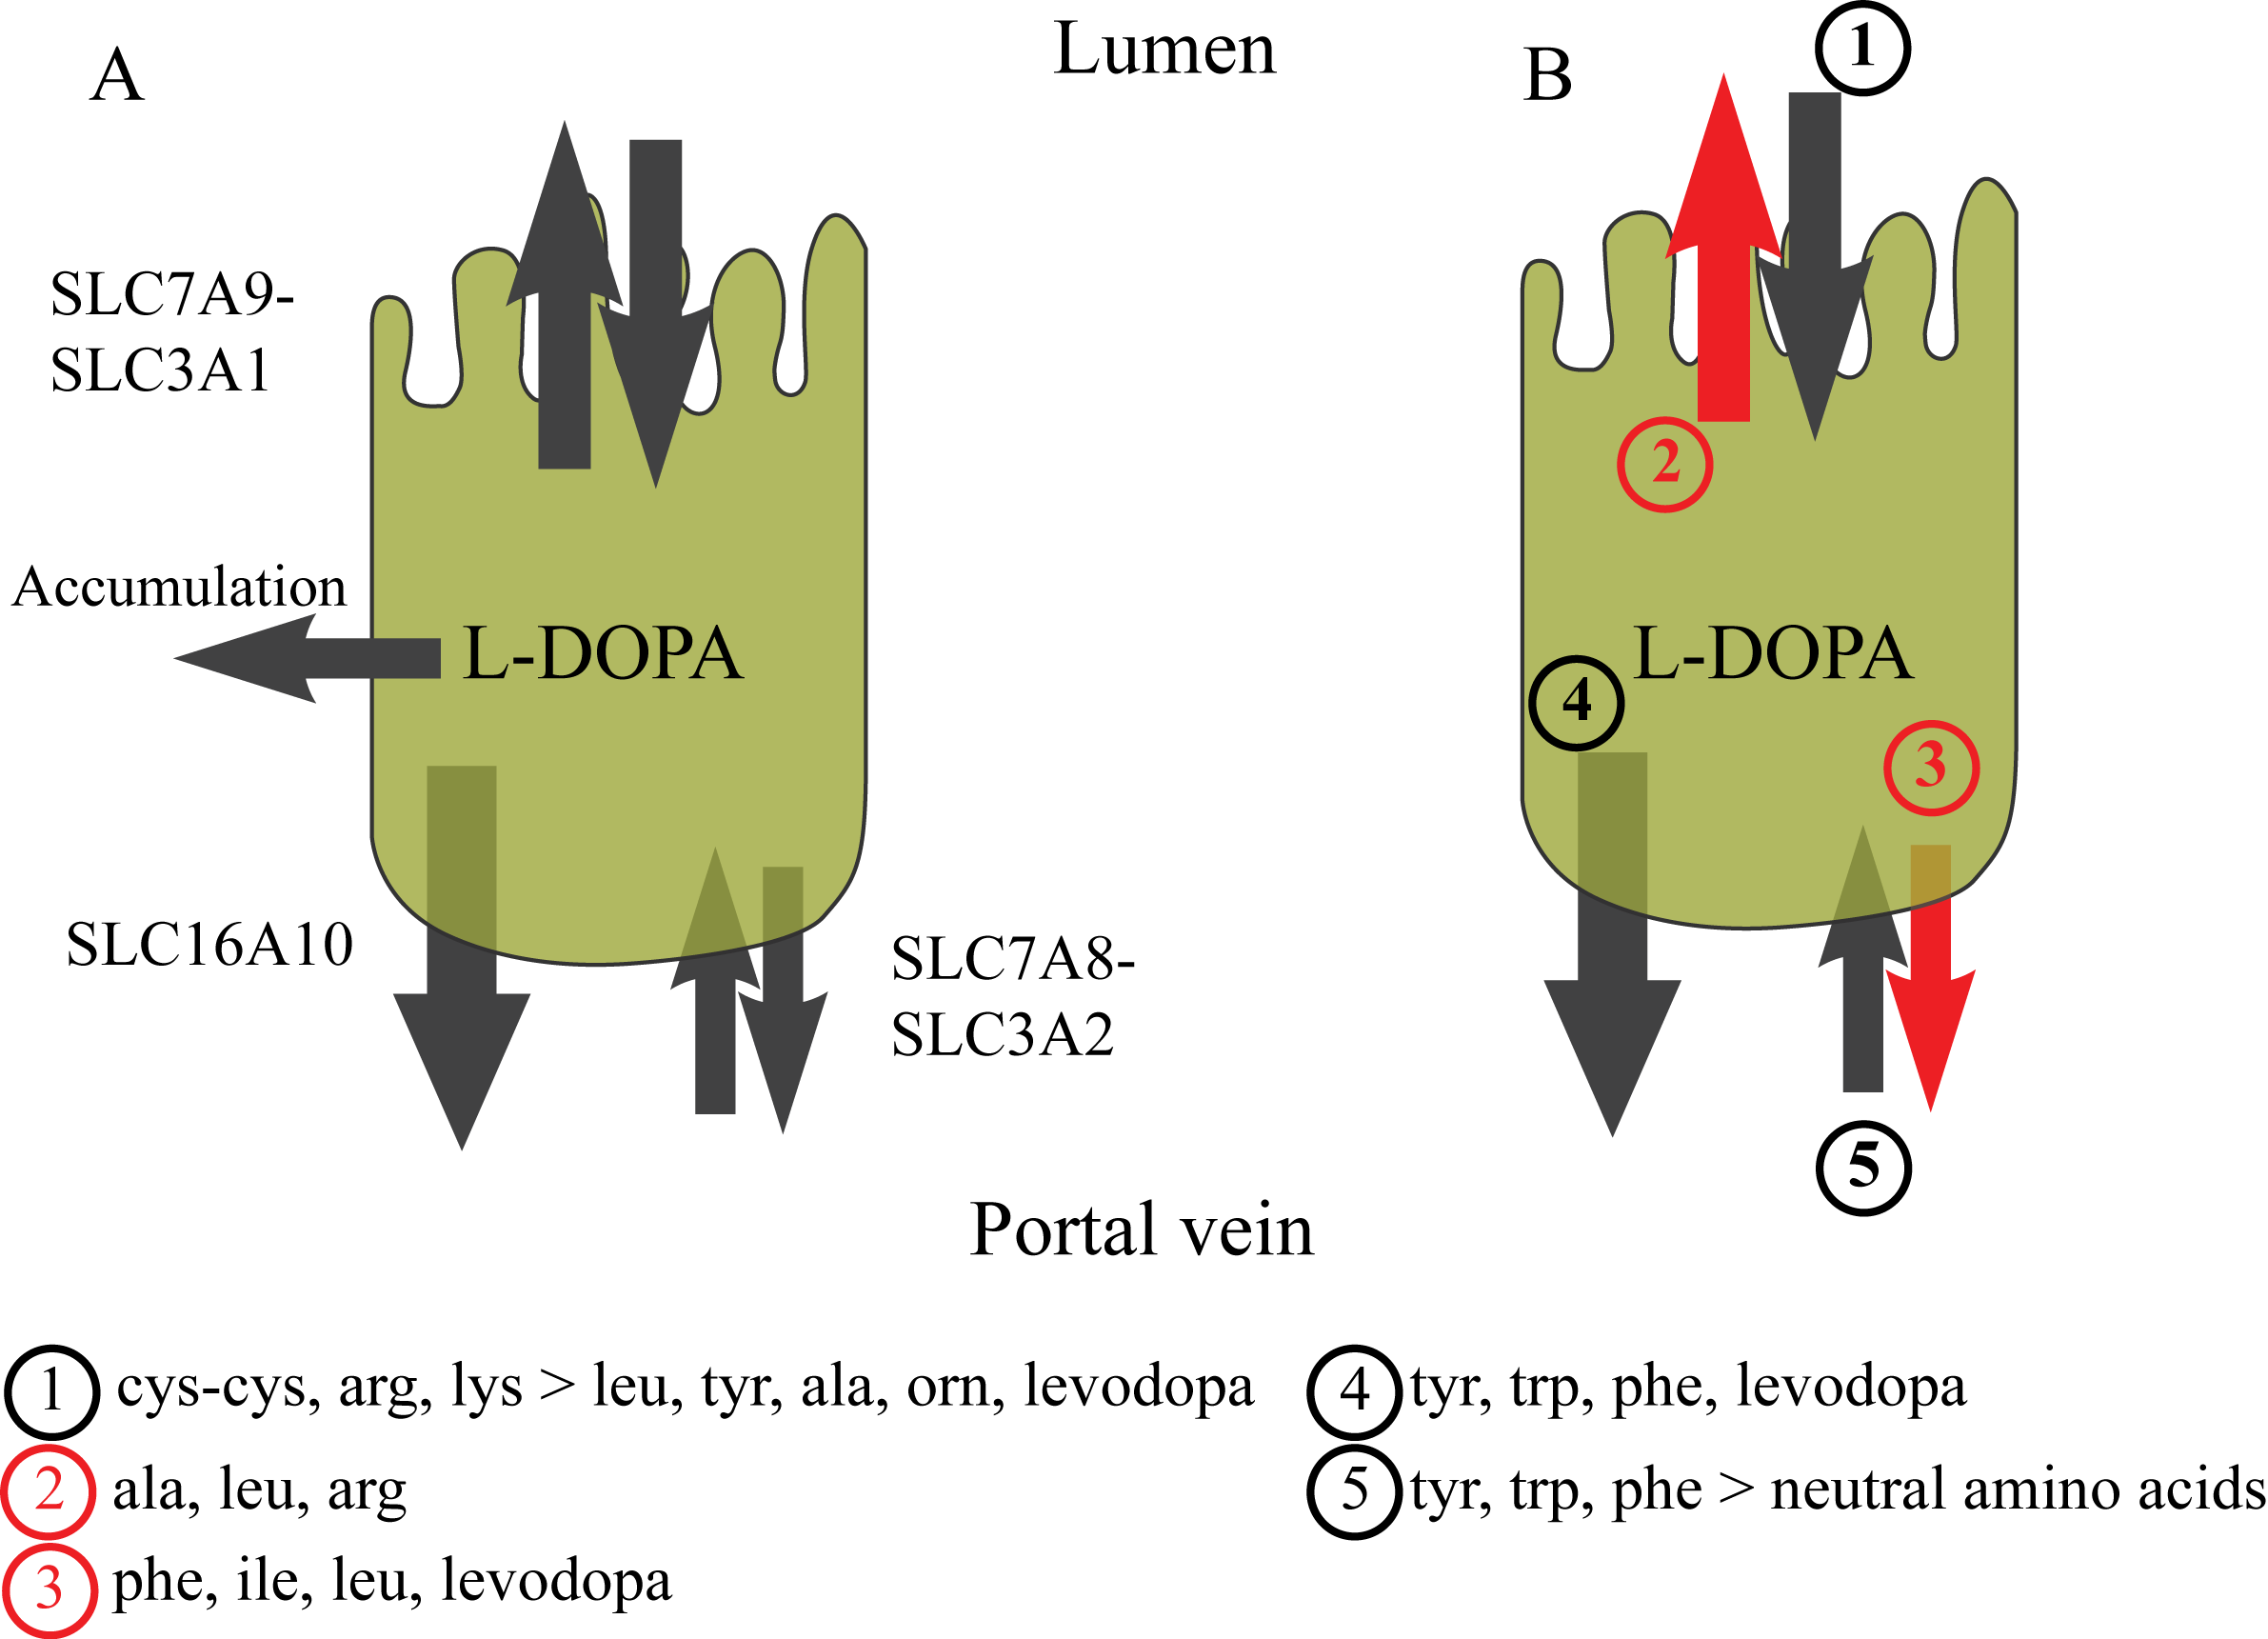
\includegraphics[width=\textwidth,height=\textheight,keepaspectratio]{GIM/figure2.png}%Figure from images\Figure1.png
	\caption[Differential metabolic fluxes between T1D and healthy.]{The multi-scale whole-body model identified disrupted metabolic processes in type 1 diabetes mellitus. A- Flux variability analysis of the pancreas in Harvey in comparison to dHarvey in healthy and type 1 diabetes models. B-Time course of glucose in peripheral blood in intravenous glucose tolerance test modeled by Harvey alone and GIM alone, and ATP theoretical amount in the adipocyte during the IVGTT as predicted by dHarvey. C-volcano plot of differential reaction fluxes (ratio of fold change) in healthy and type 1 diabetes model. D-Differential flux distribution by organ and E- by subsystem (p<0.05).}
	\label{fig:GIM2}
\end{figure}
%\cite{kuleshov2016enrichr, chen2013enrichr} Enrichr citation
In order to capture the non-glycolytic, off-target effects of T1D, we constrained the reaction fluxes in dHarvey by the gene expression of T1D human pancreas and pancreatic islets \cite{planas2010gene}. The differentially expressed set of metabolic genes (Table \ref{GIM:tbls1}) were mapped to Harvey (Figure \ref{fig:s2GIM}) alongside the target effects that were modeled with the constraints arising from GIM. The enriched terms of the selected metabolic genes (Figure \ref{fig:s0GIM}) showed that a large part of the common features of the disrupted processes in diabetes was correctly captured ( in HumanCyc \cite{romero2005computational} and the dbGap \cite{mailman2007ncbi} databases) but also represented shared feature with glucose-involving conditions (Figure \ref{fig:s0GIM}) such as malaria \cite{ogetii2010hypoglycaemia} and type 2 diabetes (in OMIM database) \cite{mailman2007ncbi}.\\
Using flux variability analysis \cite{mahadevan2003effects}, we compared the flux span of pancreatic reactions in unconstrained Harvey and dHarvey model. Harvey had a reduced solution space (Figure \ref{fig:GIM2}-A), as depicted by the flux span, when coupled to GIM. Therefore, the set of obtained solutions is constrained to biologically relevant phenotypes with respect to glucose metabolism. The T1D dHarvey model showed a smaller flux span in comparison to the dHarvey healthy model  (Figure \ref{fig:GIM2}-A), thus a decreased metabolic flexibility and adaptive behaviour towards increased glucose levels and the reduced insulin secretion that shape the disease pathophysiology.
We compared the predictive capabilities of each of Harvey, GIM, and dHarvey with respect to metabolite dynamics in intravenous glucose tolerance test (IVGTT). While GIM natively predicted glucose kinetics with top-down estimated parameters from \textit{in vivo} measured concentrations \cite{schaller2013generic}, Harvey alone fails to predict the glucose dynamics because of lack of insulin and glucagon regulation (Figure \ref{fig:GIM2}-B). dHarvey performs equally well as GIM and is able to predict the dynamics of metabolites involved in imbalanced reactions such as the ATP demand in the adipocyte during IVGTT.\\ 
The baseline glucose levels in healthy and T1D GIM models were as well coupled to Harvey and informed about steady state glucose fluxes. Using dHarvey, we compared the fold change of reaction fluxes in healthy and T1D (Figure \ref{fig:GIM2}-C). FVA was done on the healthy and T1D irreversible models (where all reactions are irreversible) to guarantee positive flux values for the consequent fold change analysis. The FVA solutions were subsequently stored, resulting in 160,032 (number of reaction times two) flux values per reaction. Using the obtained data, we were able to compare flux distributions as opposed to single flux values (Text \ref{GIM:sp5}). A fold change analysis was then performed on the flux distributions.
The obtained volcano plot showed the significantly different reaction fluxes in both conditions. A total of 33,526 reactions over a total of 80,016 reactions exhibited a change in value between the conditions, of which 6,602 were increased and 15,205 were decreased significantly above 50\% (fold change greater than 1.5) of their healthy values (p<0.001). Reaction enrichment in metabolic subsystems (Figure \ref{fig:GIM2}-D) and organs (Figure \ref{fig:GIM2}-E) showed an expected systematic and ubiquitous deregulation of glucose metabolism, particularly in target organs (pancreas, liver, and kidney). 
The subsystem for transport reactions is the most affected since it covers glucose exchange from producing organs, e.g., glycogenolysis in the liver to energy-requiring processes. Overall, the differential fluxes of reactions were related to known semiology of T1D in the different organs (Table \ref{GIM:tbls4}), e.g., cardiovascular disease, retinopathy, ketoacidosis, and liver glycogen deposition. 
Of notable difference, the disruption of the transport system in T1D (Figure \ref{fig:GIM2}-E) suggested a prominent role of insulin in maintaining a global inter-organ communication. We will investigate this aspect in the next section.

\subsection{Prediction of exogenous insulin off-target effects}

\begin{figure}[!htp]
\centering
	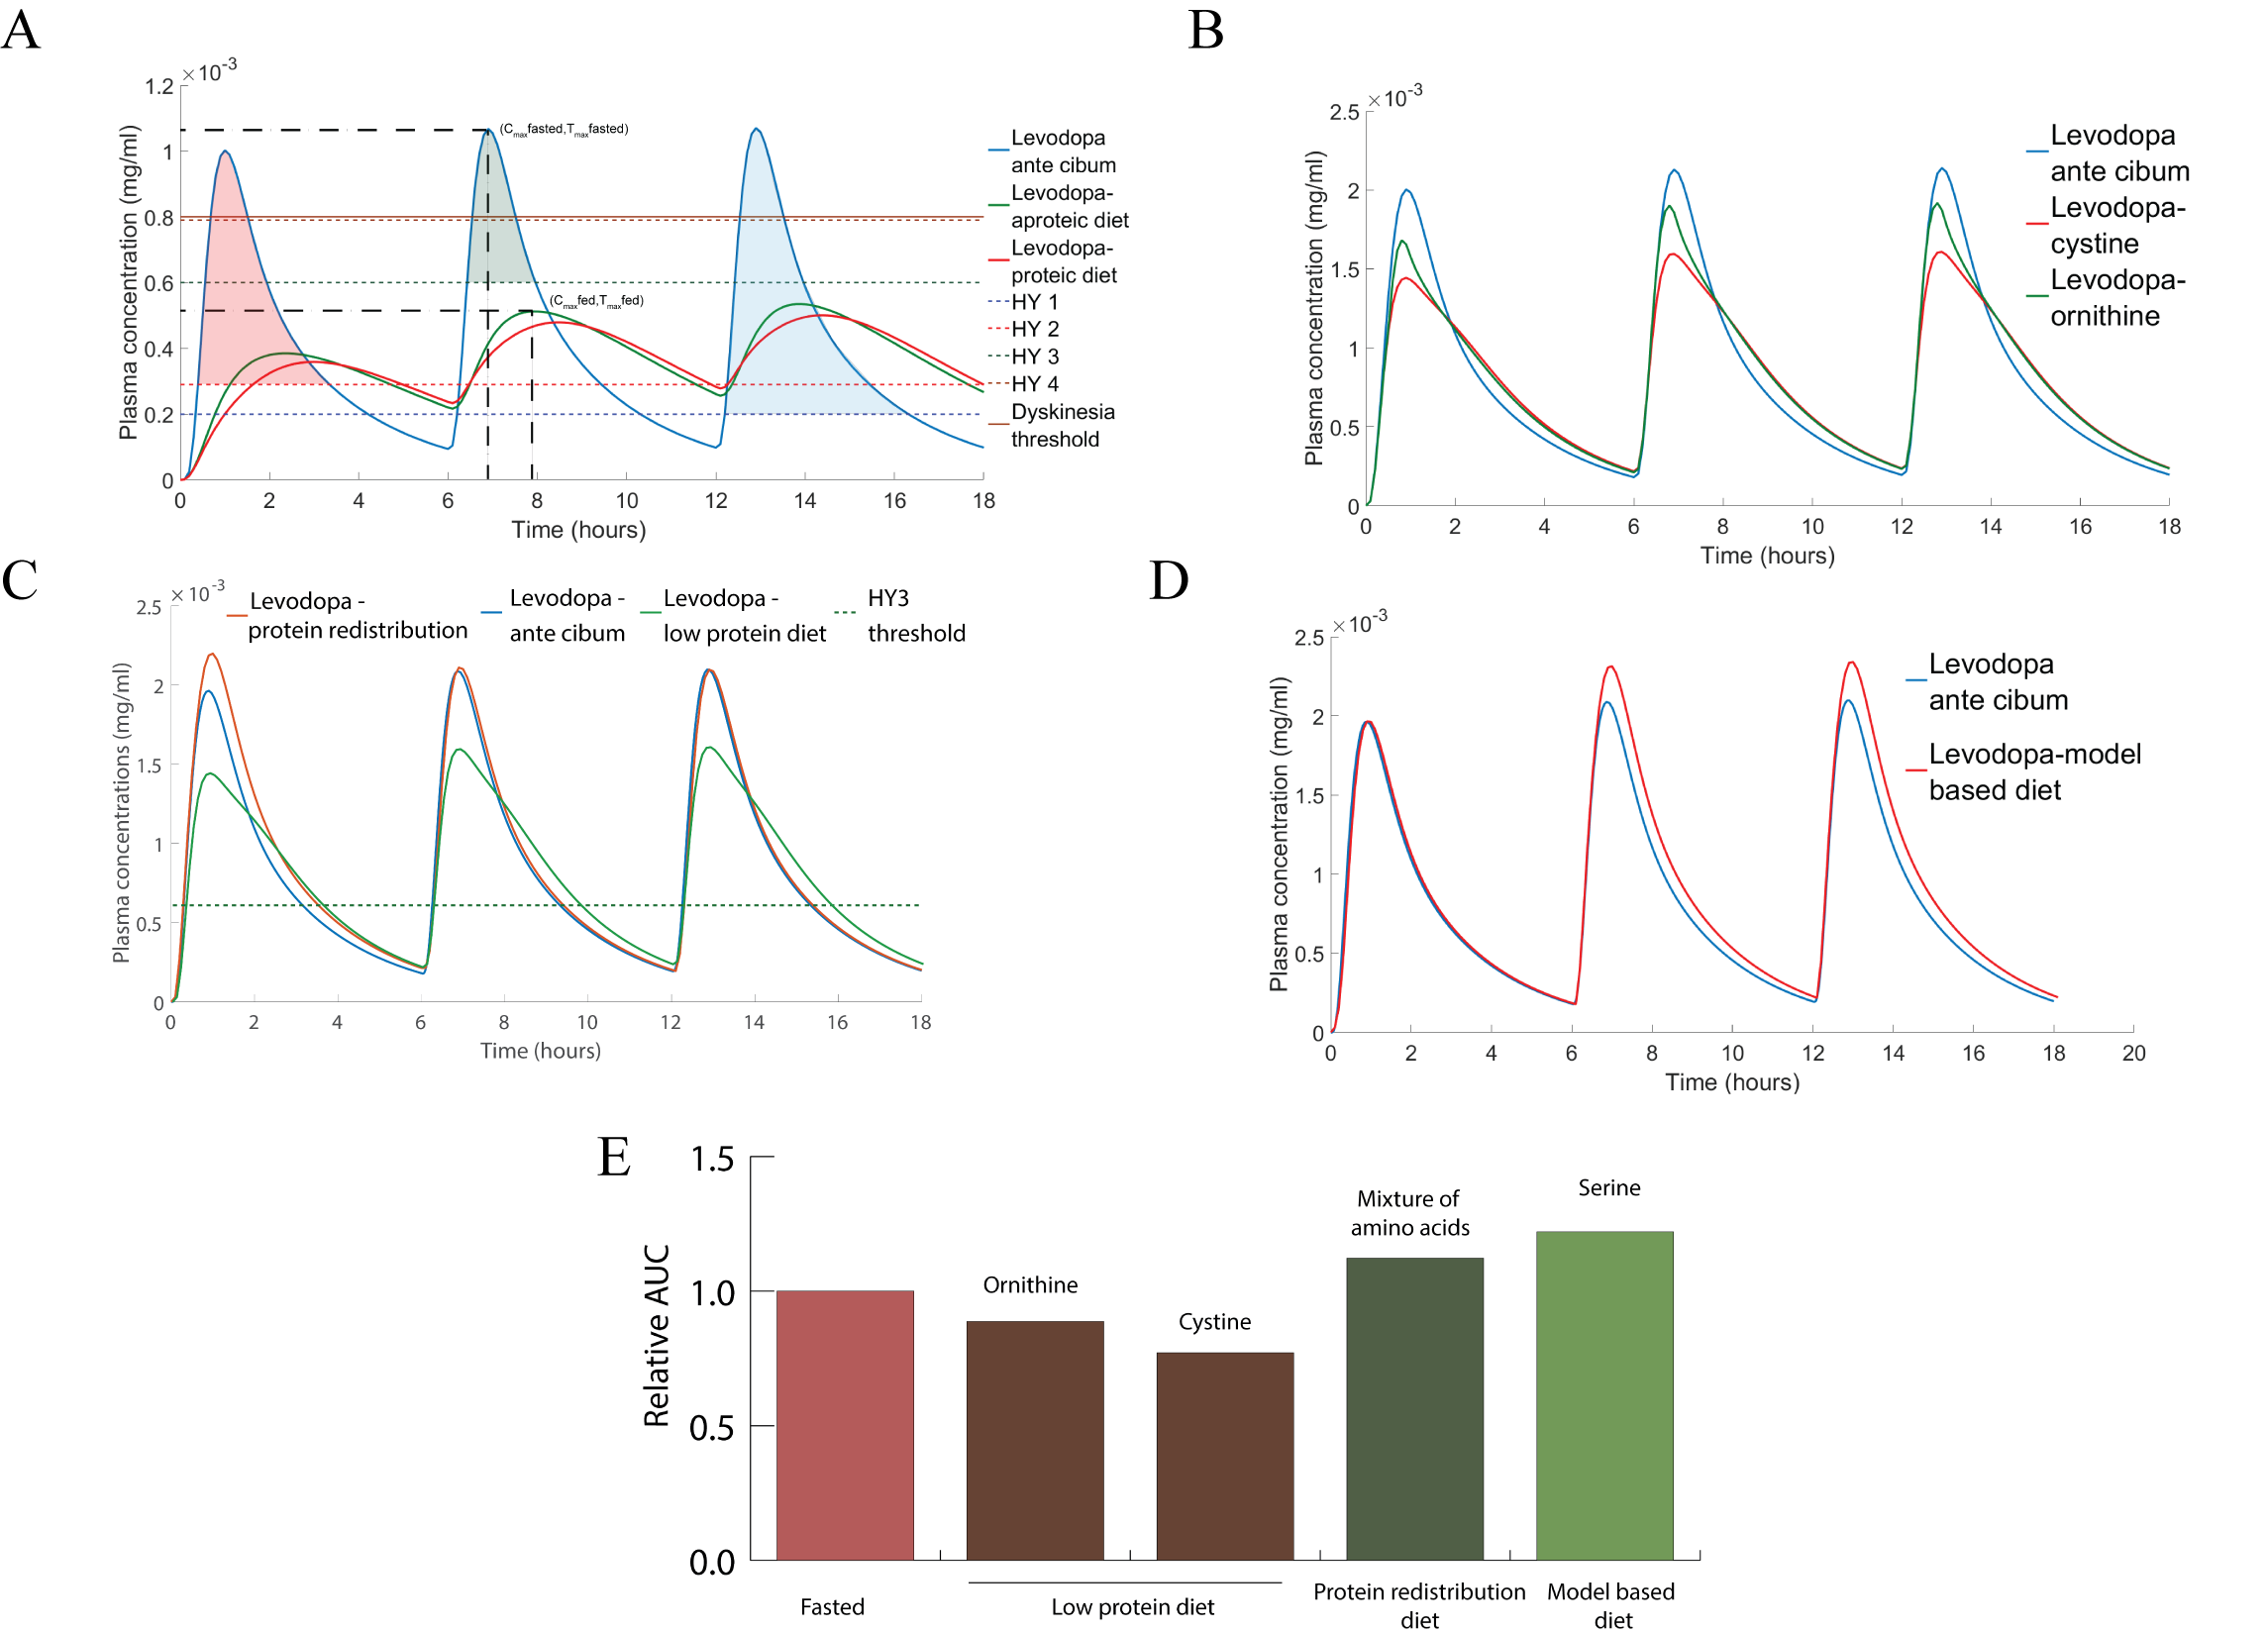
\includegraphics[width=\textwidth,height=\textheight,keepaspectratio]{GIM/figure3.png}%Figure from images\Figure1.png
	\caption[Insulin metabolic off-target effects.]{(Continued on the following page)}
	\label{fig:GIM3}
\end{figure}
\begin{figure}[t]
  \contcaption{Insulin metabolic off-target effects assessed by the probability density estimates of reaction flux values. The fluxes include A-glucose uptake, B-liver glycolytic reactions, C-metal homeostasis, D-fatty acids reactions and E-amino acids uptake, in various organs after a subcutaneous insulin administration.}% Continued caption
\end{figure}

The physiological effects of insulin mainly affect the uptake of glucose by organs. A recent study \cite{yugi2014reconstruction} suggested  a regulation of the liver isoform of phosphofructokinase (PFK) by insulin such that upstream fluxes of PFK are downregulated and downstream fluxes upregulated. Dynamics of liver glycolysis fluxes in subcutaneous insulin bolus setting (Figure \ref{fig:GIM3a}) confirmed three out of eight regulatory flux patterns, while one flux remained invariant and four were mispredicted. As this new insight was not captured in dHarvey, we used an additional dynamical model \cite{yugi2014reconstruction} to represent the off-target effects of insulin in the liver. The ODE model was coupled to dHarvey which now captures both T1D and insulin target and off-target effects. In addition to glycolysis, insulin influences amino acids uptake, particularly large and neutral ones (LNAA), resulting in a decrease in blood concentrations of LNAA. The model predicted a decrease in all LNAAs in the blood (Figure \ref{fig:GIM3a}) after 60 minutes of insulin administration, preceded by a transient increase at 30 minutes.
In order to infer the metabolic effects of insulin, interpreting single solutions of dHarvey proves ineffective given the high dimensionality of the model and the alternate optimal solution (AOS) space. To characterize the AOS space, FVA provided an empirical flux probability density per reaction. We compared the probability density estimates of the fluxe values in T1D with and without insulin administration. Glucose uptake expectedly increased in the muscle, adipocytes, and lungs while remaining unchanged in the liver and brain (Figure \ref{fig:GIM3}), as expected given their vital role. Insulin stimulated the activity of phosphofructokinase, glycogen phosphatase, and hexokinase while inhibiting glucose-6-phostphatase, contributing to its overall anabolic effect. The uptake of phosphate by the adipocytes also increased, which links to the known depletion  of metals after continuous insulin injection, while the uptake of potassium did not change significantly. In relation to the fatty acids biosynthesis, insulin enhanced the synthesis of lipoproteins in the liver, inhibited the oxidation of fatty acids and the diacyl glycerol lipase in the adipocytes. The prediction of triglycerides levels using CRONICS (Figure \ref{fig:GIM3b}), showed an increase in the adipocytes following the administration of insulin. Finally, the uptake of glutamine in the red blood cells and serine in the spleen, taken as example (Figure \ref{fig:GIM3}), supported our findings regarding the higher insulin-induced uptake of amino acids.\\
Moreover, we investigated the anabolic effect of insulin on inter-organ crosstalk. Due to large running times, the simulation of the dHarvey model using CRONICS framework restricted the distance minimization of the flux vectors between the different time steps (Figure \ref{fig:s3GIM}-step VI) to a subvector including pancreas, kidney, adipocytes, muscle, liver, brain, and fluids, e.g., peripheral blood, portal vein, blood brain barrier, intestinal compartments. The comparison of the inter-organ crosstalk in dHarvey after insulin administration to the T1D steady state showed an increase in the metabolites exchange set, particularly in the muscle, kidney, brain, and liver (Figure \ref{fig:GIM3c}). The total number of exchanged metabolites in T1D model equalled 229 exchanged metabolites while insulin induced an exchange of 297 metabolites overall. 
Finally, having constructed dHarvey, a dynamical hybrid model of type 1 diabetes and insulin response, we investigated the effects of within and between patient response to insulin administration.
\subsection{Between-subject variability is reflected in citric acid cycle and oxidative phosphorylation}
Using the dHarvey model representing both T1D and insulin target and off-target effects, we investigated the mechanisms underlying inter-individual variability. A set of kinetic parameters of the GIM model with differential values in T1D and healthy individuals (Table \ref{GIM:tbl1}) \cite{schaller2013generic} was varied (Figure \ref{fig:GIM4}-A) to reproduce the clinically observed 25-35\% \cite{heinemann2002variability} of inter-individual variability in 31 synthetic type 1 diabetes patients (30 simulated patients and 1 reference average patient) (Figure \ref{fig:GIM4}-B). The obtained between-subject variability equalled 30.11\%, in agreement with the empirical values. For every synthetic patient, the personalized dHarvey was simulated for 600 minutes after the subcutaneous injection of insulin bolus.\\
\begin{table}[!htp]
\caption[Selected whole-body parameters in inter-individual variability simulations.]{Selected whole-body parameters in inter-individual variability simulations.}
\begin{center}
	\begin{tabular*}{\textwidth}{l @{\extracolsep{\fill}} ll}
	\hline
	Parameter & GIM path  & Description         \\ 
	\hline
	P\_1711    & Liver|Interstitial|Glucagon\_0 & Baseline glucagon level in the liver   \\
	P\_2049    & Pancreas|Interstitial|Insulin\_0 & Baseline insulin level in the pancreas \\
	P\_322          & Fat|Endosome|End\_IR\_0 & Adipocyte baseline insulin receptor \\
	& & in the endosome \\
	P\_1757/P\_1755  & Liver|Intracellular|End\_IR\_0\_liv & Liver baseline insulin receptor in the cell \\
	P\_1978 & Muscle|Endosome|End\_IR\_0  & Muscle baseline insulin receptor in\\
	& & the endosome      \\
	P\_323          & Fat|Endosome|End\_IRp\_0  & Adipocyte baseline insulin phosphorylated\\
	& & receptor in the endosome        \\
	P\_1760         & Liver|Intracellular|End\_IRp\_0\_liv & Liver baseline insulin phosphorylated\\
	& & receptor in the cell \\
    P\_1979 & Muscle|Endosome|End\_IRp\_0        & Muscle baseline insulin phosphorylated\\
    & & receptor in the endosome     \\
    P\_293            & Fat|Intracellular|IR\_cell\_0 & Total concentration of adipocyte\\
    & & intracellular insulin receptor \\
    P\_1753          & Liver|Intracellular|IR\_cell\_0 & Total concentration of liver intracellular\\
    & & insulin receptor   \\
	P\_1950    & Muscle|Intracellular|IR\_cell\_0 & Total concentration of muscle intracellular\\
	& & insulin receptor \\
	P\_294          & Fat|Intracellular|IR\_p\_0 & Adipocyte baseline insulin phosphorylated\\
	& & receptor in the cell   \\
	P\_1758/P\_1727            & Liver|Intracellular|IR\_p\_0 & Liver baseline insulin phosphorylated  \\
	& & receptor in the cell \\
	P\_1949 & Muscle|Intracellular|IR\_p\_0 & Muscle baseline insulin phosphorylated       \\
	& & receptor in the cell \\
	P\_1814          & Liver|ReceptorRecyclingFactor-End  & Liver receptor recycling factor\\
	& & in the endosome        \\
	P\_1994         & Muscle|ReceptorRecyclingFactor & Muscle receptor recycling factor \\
    P\_338 & Fat|ReceptorRecyclingFactor        & Adipocyte receptor recycling factor     \\
    P\_1811            & Liver|ReceptorRecyclingFactor & Liver receptor recycling factor \\
	\hline
	\end{tabular*}
\end{center}
\label{GIM:tbl1}%descriptive label to refer to figure in text
\end{table}
The distribution of active reactions across patients and across time was very similar (Figure \ref{fig:GIM4}-C, Figure \ref{fig:s4GIM}), which indicated a similar metabolic network topology. Reducing the dimensionality of flux distribution through PCA (Figure \ref{fig:GIM4}-D) showed that the observed change is driven by the modulation of reaction flux values across time following the action of insulin. Particularly, the end metabolic state was different than the initial state, confirming a metabolic change as an action of insulin. Moreover, each individual had a differential metabolic shift reflective of a quantitative variation in flux values across pathways (Figure \ref{fig:GIM4}-E). Interestingly, we observed that insulin exerted a hysteresis between peripheral glucose concentrations and whole-body metabolism (Figure \ref{fig:GIM4}-F), that was achieved differently between the different individuals.\\
Additionally, we investigated the impact of inter-individual variability on the different metabolic pathways. Particularly, pentose phosphate pathway and glycolysis were remarkably robust towards insulin-induced perturbation, while citric acid cycle and oxidative phosphorylation total whole-body flux over time showed a patient-specific variation (Figure \ref{fig:GIM4}-G). Furthermore, we investigated the effect of intra-individual variability to insulin response on whole-body metabolism.
\subsection{Within-subject variability to insulin}
\begin{figure}[!htp]
\centering
	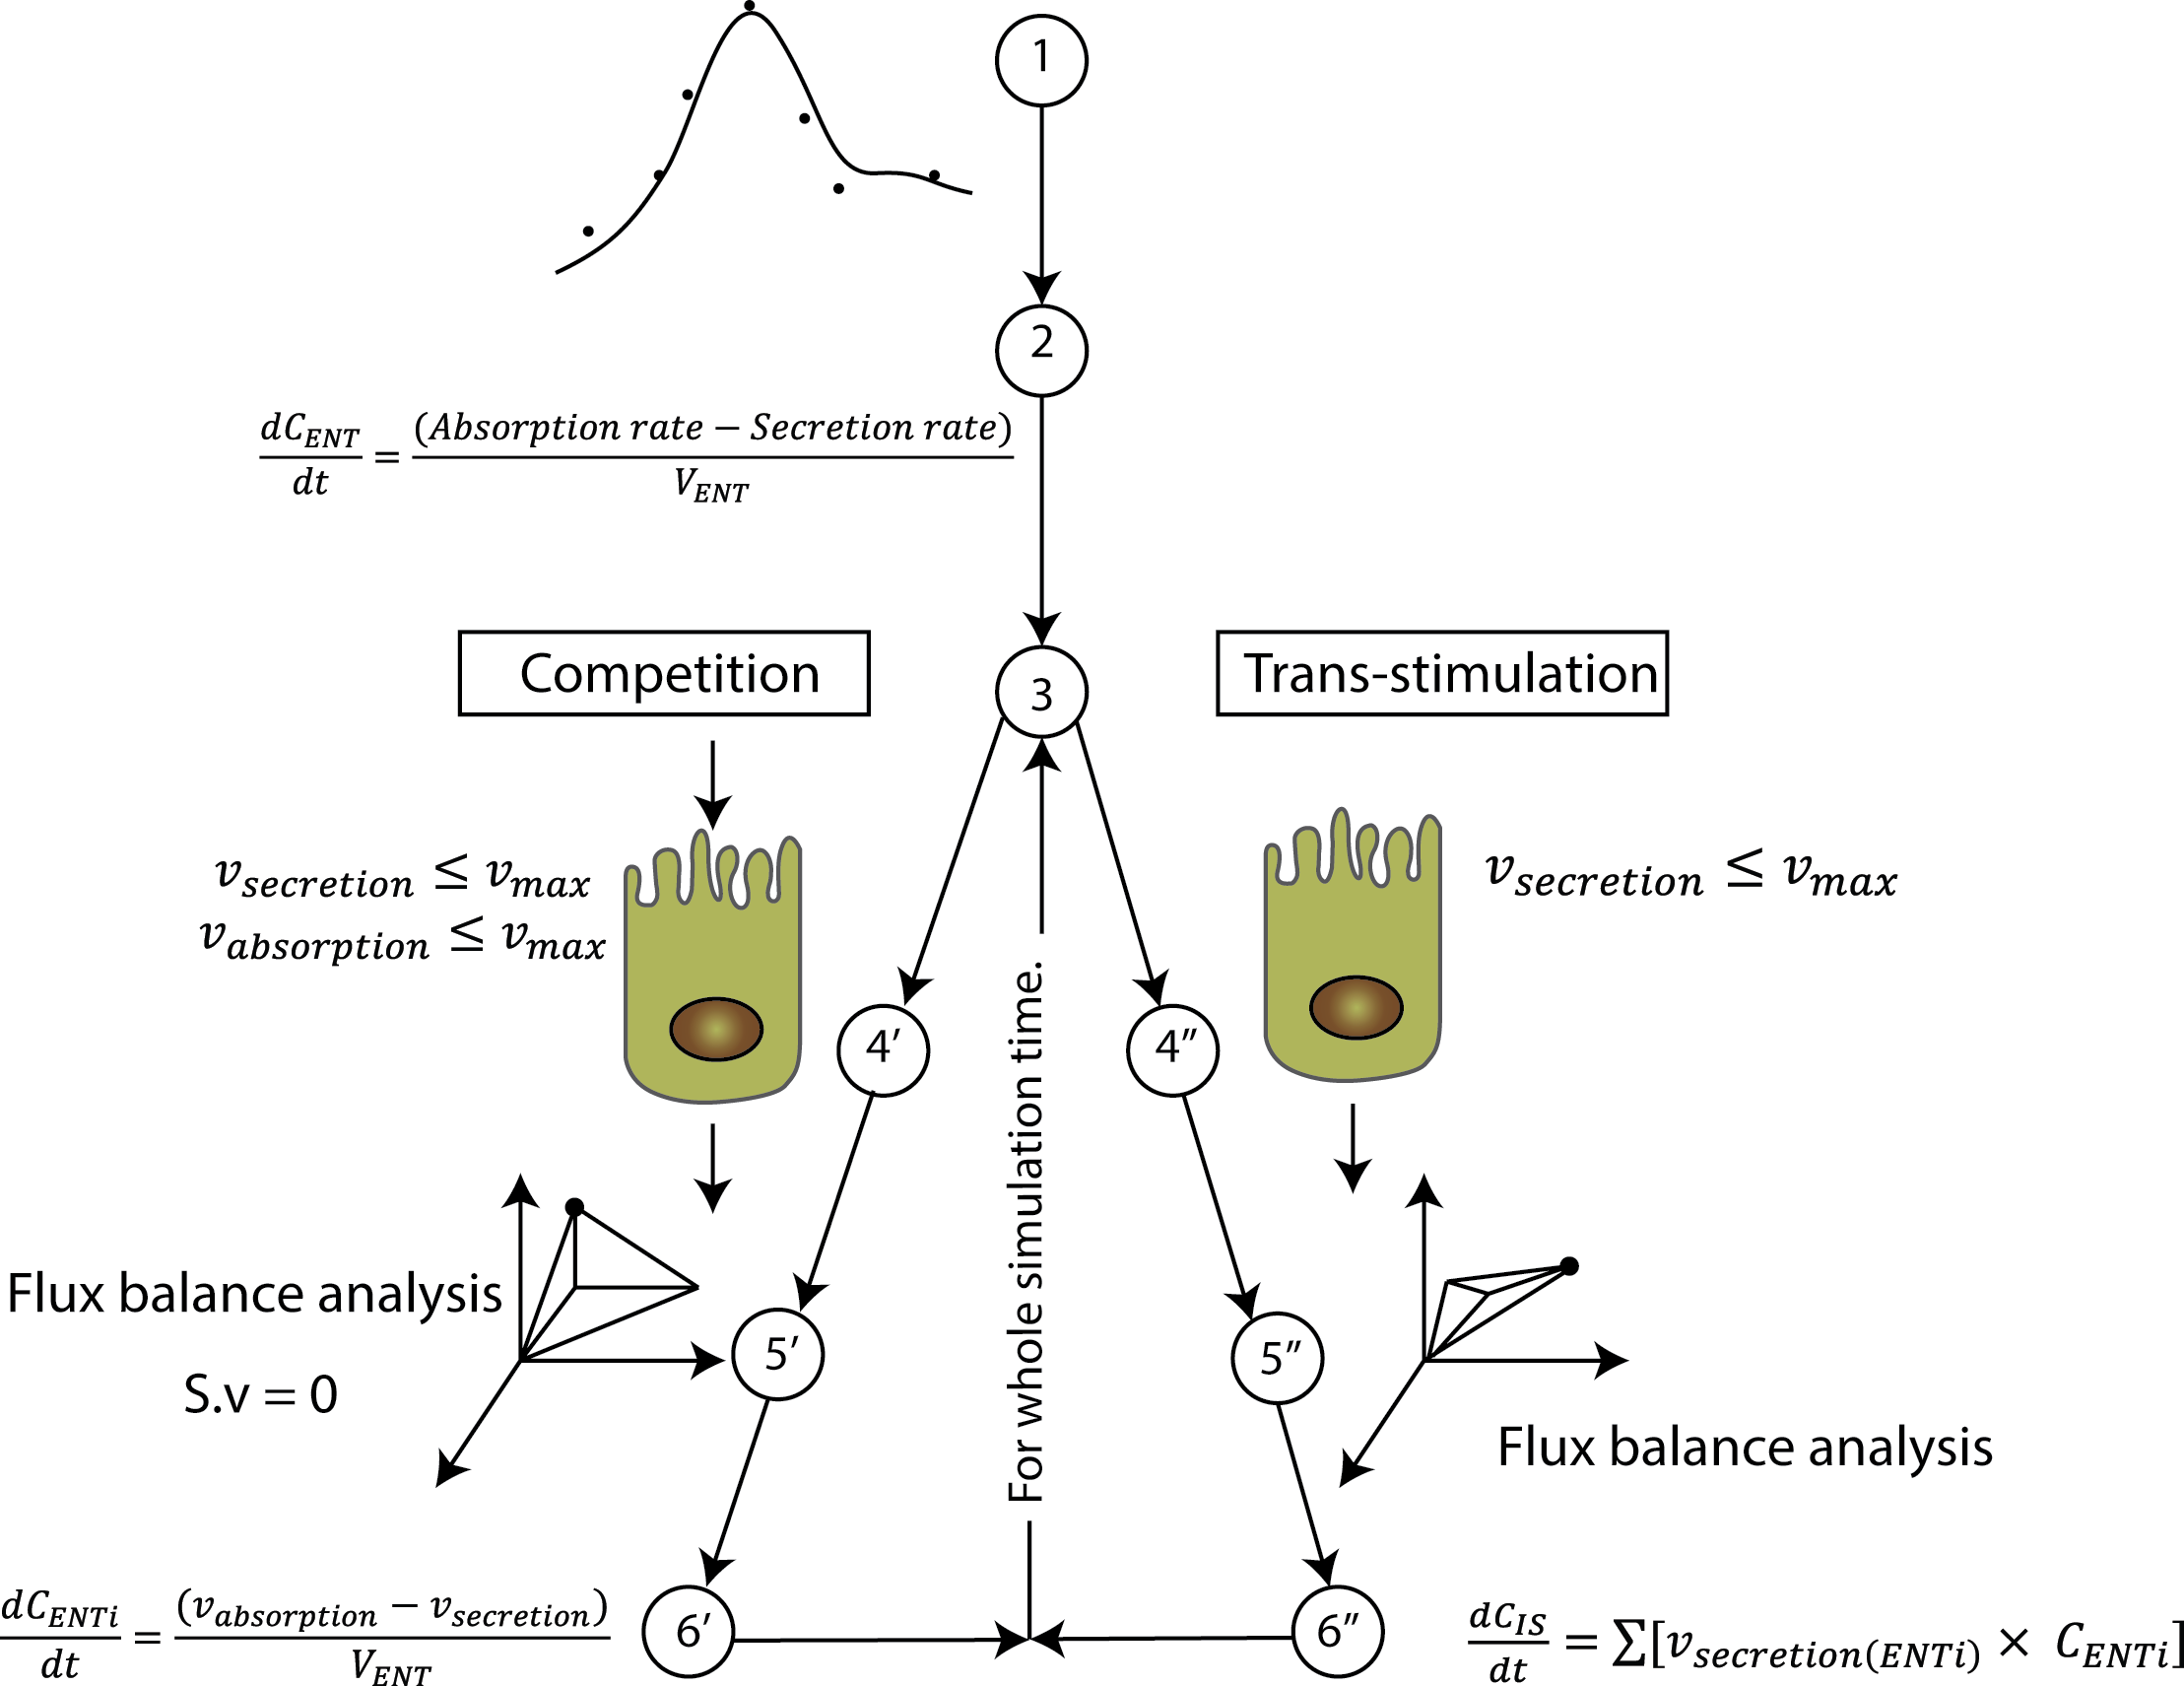
\includegraphics[width=\textwidth,height=\textheight,keepaspectratio]{GIM/figure4.png}%Figure from images\Figure1.png
	\caption[Inter-individual variability to insulin response.]{(Continued on the following page)}
	\label{fig:GIM4}
\end{figure}
\begin{figure}[t]
  \contcaption{Inter-individual variability to insulin response is reflected on key pathways of metabolism. A- Varying a set of individual parameters within the reported inter-individual variability range in the dynamical model yields B- different peripheral glucose concentrations as a response to insulin injection. C- Distribution of the active reactions over simulation time per patient. D- Evolution of the metabolic fluxes as represented by PCA over simulation time of the average patient (patient 1) and E- the population of synthetic patients. F- Insulin-induced hysteresis between glucose peripheral blood levels and whole-body metabolism. G- Citric acid cycle and oxidative phosphorylation total flux reflect between-patient variability while glycolysis and pentose phosphate pathways are stable to perturbation. The flow chart was done using Rawgraphs \cite{Mauri:2017:RVP:3125571.3125585}.}% Continued caption
\end{figure}
Within-subject variability to insulin results from internal, endogenous factors that are specific to a particular metabolic state of the individual, e.g., postprandial state, physical activity. In order to determine the influence of the metabolic state on peripheral glucose dynamics, we set the kinetic parameters of the simulated patient to the reported population mean in GIM and varied the metabolic reactions. In each metabolic state, we generated random objective coefficient weights to every reaction (Figure \ref{fig:GIM5}-A). The weights could be lower, higher, or equal to the mean profile. In the latter case, the simulated profile approached the predictions of the GIM model. To each set of internal perturbations (input) to metabolism, i.e., increase or decrease in reactions weights, we measured the minimal glucose concentration and the final concentration after 10 hours of subcutaneous insulin injection (output) \cite{sarkar2010regression}. In all cases, the time step was decreased from five minutes to 2.5 minutes as both integration failures and conflicting constraints arose from higher time steps.  In the described setting, the reactions of dHarvey fell under two classes, the reactions proper to Harvey and those shared by both GIM and Harvey, referred to as interface reactions \cite{wadehn2016multiscale}. Changing the coefficients of the interface reactions only and simulating dHarvey with FBA for 10 metabolic states resulted in a smooth set of glucose dynamics (Figure \ref{fig:GIM5}-B). In order to get a complete view of the within-patient variability, the reactions proper to the Harvey were included as well. Using FBA to simulate 10 metabolic states of the hybrid model, the glucose profiles showed non smooth profiles, with non-biological concentrations or terminated in the course of simulation (Figure \ref{fig:GIM5}-C).  Finally, performing the simulation using CRONICS ensured both smoothness of the system and minimal debugging to resolve conflicting constraints (Figure \ref{fig:GIM5}-D), of which only 2 simulations permanently failed as they have reached a null concentration of glucose and were removed from subsequent analysis. The 29 metabolic states simulated with the final setting resulted from the perturbation of a total of 2817 reaction. Each metabolic state consisted of a set of perturbed reaction activity as depicted by the random coefficient matrix (Figure \ref{fig:GIM5}-E).
The computed intra-individual variability equalled 30\% \textit{in silico} and was in agreement with the empirical value of 12-45\% \cite{heinemann2002variability}. To determine the influence of every reaction to the metabolic profile of glucose, a multivariate regression was performed using the coefficients matrix as input and a matrix of glucose concentrations per state as output. The minimal and final glucose concentrations were considered for the sensitivity analysis as they inform about adverse reactions and treatment efficacy, i.e., hypoglycemia and hyperglycemia. The reaction sensitivities to both of the readouts (Figure \ref{fig:GIM5}-F) showed that GLUT4 transport had a great share of the influence on glucose profile. Interestingly, reactions from the bile acid synthesis pathway modulated the peripheral glucose profile as well.  Taken together, these findings showed that internal reactions in Harvey, that were not in necessarily in the interface reactions set, had the potential to modulate the glucose concentrations in GIM, through glycolytic and non-glycolytic pathways, thereby suggesting novel approaches to achieve diabetes control.
\section{Discussion}
We developed a multi-scale, dynamic, and organ-resolved model through multi-algorithm integration of metabolic and regulatory processes in T1D. The short time scale insulin-glucose-glucagon regulatory dynamics (GIM) served as constraints to the whole body metabolic network (Harvey). In addition to the expected target effects, the mechanism-unrelated metabolic effects of both insulin and type 1 diabetes pathophysiology were included in the model through organ-specific gene expression data and metabolomics time-course. The integrative model provided a complete picture on the network dynamics, regulation, and response to perturbation and links it to known symptoms and clinically relevant variability of insulin response both within and between-subject.  
\subsection{Chronic inflammation in type 1 diabetes improves disease identification using whole-body fluxes}
In order to assess the impact of the tolerance tests on the whole-body level, the metabolic model (Harvey) was constrained by the glucose-insulin-glucagon regulation modelled by GIM in insulin and glucose challenges involving healthy and T1D states. The metabolic fluxes were consequently used as features in an SVM binary classifier \cite{shaked2016metabolic}. Identifying insulin versus glucose challenges at five minutes and 15 minutes after perturbation was possible due to the opposite effects that these substances induced on the human body (Figure \ref{fig:GIM1}-C). The identification of healthy and T1D flux distribution improved the separation between healthy and T1D individuals after the addition of gene expression constraints in T1D, representing the chronic inflammation that triggers the pathogenesis of the disease. While glycaemia control is achieved through allopathy, the inflammatory aspect of the disease is often overlooked \cite{mccall2013treating} and has to be equally addressed. In addition, it was possible to define a healthy and diabetic boundary using whole-body metabolic fluxes despite the subjected constraints affected mainly the glucose-related pathways (Figure \ref{fig:GIM1}-D). These findings further reinforce the idea that type 1 diabetes is a multifactorial, pan-organ and systemic disease because of the key role that glucose plays in regulation of metabolism and energy.
\subsection{Differentially regulated fluxes suggest mechanisms underlying the systemic symptomatology of type 1 diabetes}
\begin{figure}[!htp]
\centering
	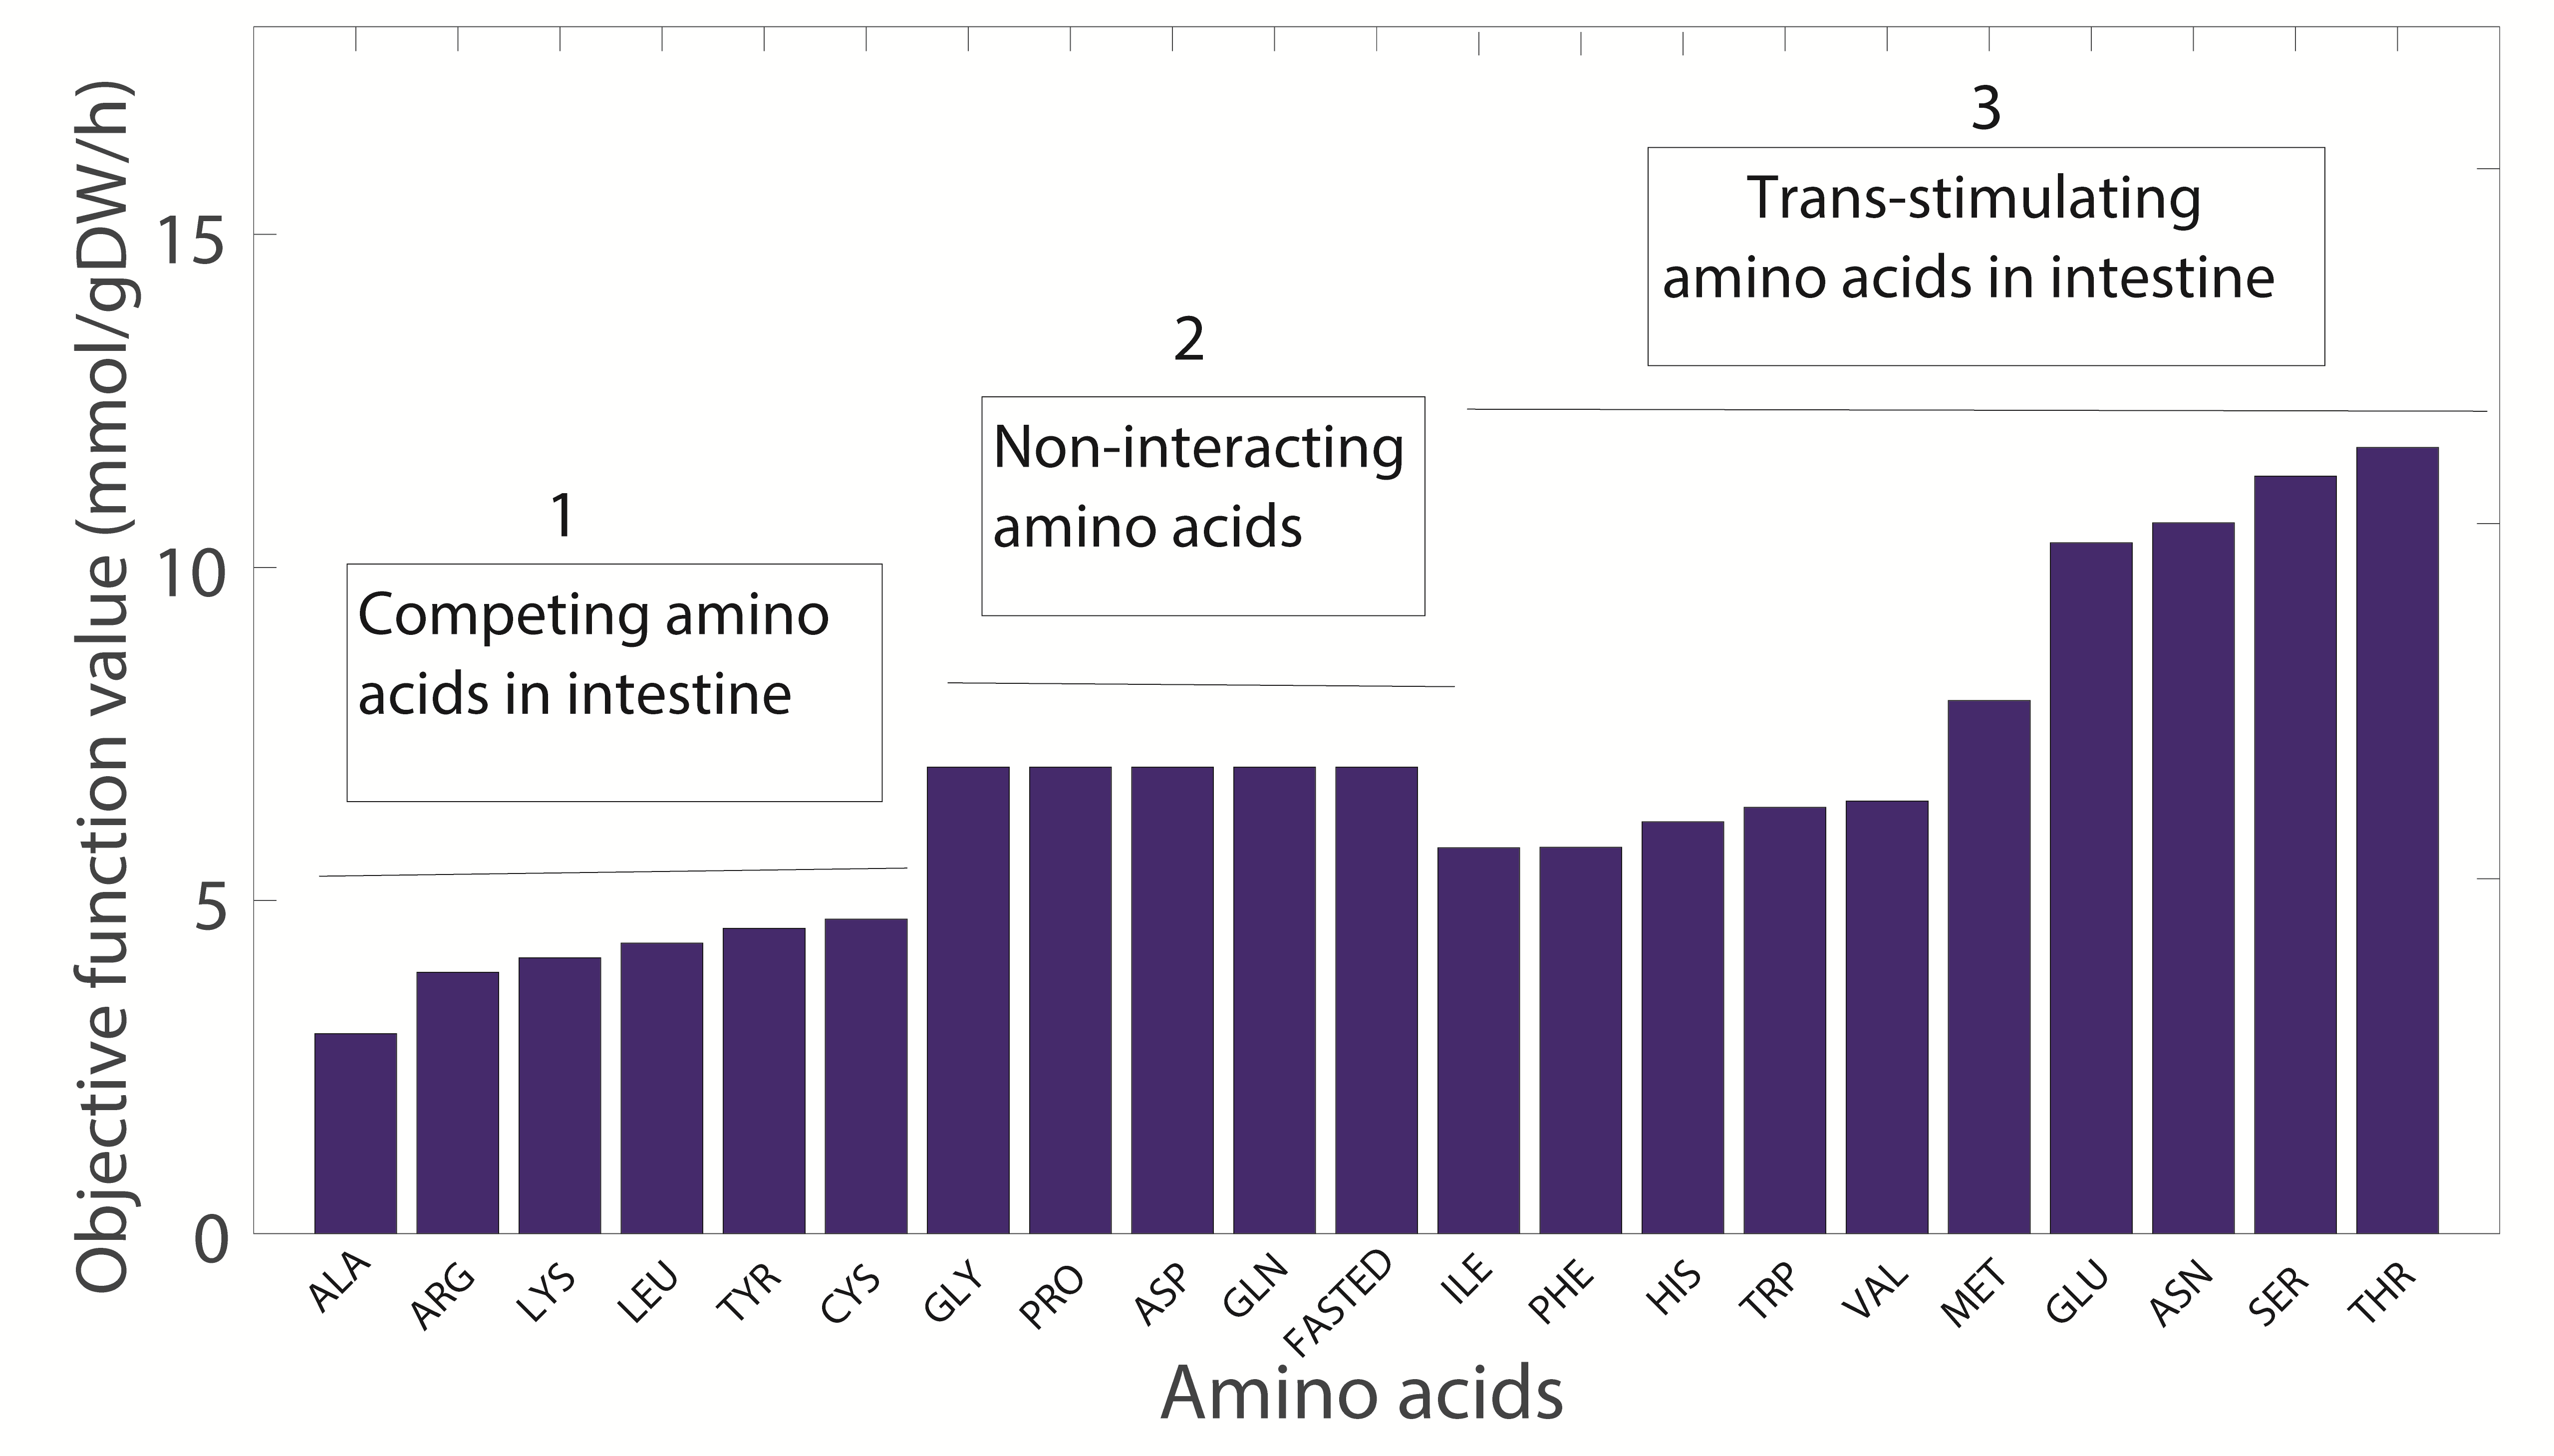
\includegraphics[width=\textwidth,height=\textheight,keepaspectratio]{GIM/figure5.png}%Figure from images\Figure1.png
	\caption[Intra-individual variability to insulin response.]{(Continued on the following page)}
	\label{fig:GIM5}
\end{figure}
\begin{figure}[t]
  \contcaption{Intra-individual variability is assessed through sensitivity analysis of the integrated model. A- The method consists of assigning random objective coefficients to metabolic reactions and measuring the minimal and final concentration of glucose for every state with the kinetic parameters set for the population mean. B-Peripheral glucose profile when only the interface reactions are varied, the simulation is carried with FBA (n=11). C-Glucose profile when both the interface reactions and the metabolic model reactions are varied, using FBA (n=11). D-Glucose profile when both the interface reactions and metabolic model reactions are varied, using CRONICS (n=31). E- A 31-column excerpt of the matrix of variation of reaction weights in the objective for every state. The total number of reactions considered was 2817. F- Computed sensitivities of every reaction in the internal state to the external output (minimal and final concentration of peripheral glucose). The reactions are described in table \ref{GIM:tblsRxn}.}% Continued caption
\end{figure}
We used gene expression data from type 1 diabetic pancreatic islets as constraints to represent the pathophysiology of the disease that associated both the chronic inflammation and the disruption of glycolytic processes. The total number of metabolic reactions in T1D was the same in the healthy model as no evidence suggested complete metabolic gene knockout in affected patients. dHarvey predicted a decrease in ATP in adipocyte (Figure \ref{fig:GIM2}-B) following the IVGTT test as glycogen storage pathways are activated over ATP producing pathways. 
Significantly  decreased pathways in T1D encompass mostly transport pathways in relation with the pan-organ distribution of insulin and the systemic properties of the disease. The well-known switch to fatty acid synthesis in type 1 diabetes is demonstrated in enrichment of the corresponding pathways (Figure \ref{fig:GIM2}-E). The up-regulation of sphingolipids, has been linked in particular to a decrease in tissue insulin sensitivity \cite{russo2013sphingolipids} in metabolic disorders and obesity.\\
Interestingly, tyrosine metabolism is significantly ranked in the up-regulated processes in T1D (Figure \ref{fig:GIM2}-E), and recent studies have found direct links between diabetes and tyrosine pathway disruption \cite{ferguson2013tatn}. Additionally, the alteration of the phosphoinositide metabolism was reported in a streptozotocyin-induced diabetes in platelet cells \cite{jethmalani1994platelet}. 
Moreover, the glycosaminoglycan family (chondroitin, keratin sulfate and N-glycan) which include naturally occurring molecules maintaining the tissue and cartilage, are decreased in T1D and could be at the origin of long-lasting manifestations such as the well-known disruption of tissue structure, e.g., diabetic foot. A study in rats showed a decrease of chondroitin sulfate in the kidney suggesting a possible implication in diabetes induced nephropathy \cite{joladarashi2011diabetes}. Collectively, the down-regulation of tissue remodeling pathways adds further evidence to the observed eschar-related symptomatology in diabetes. Since these manifestations happen at later stages, the tissue remodeling pathway \cite{gowd2016glycosaminoglycan} could be considered for interventional (either allopathic or nutritional) targets in the diagnosis phase.\\
The enrichment of genes associated to the increased fluxes in T1D (Table \ref{GIM:tbls2}) showed a representation of classical pathways such as the oxidative phosphorylation and carbon metabolism and, interestingly, Alzheimer's disease (AD), and Parkinson's disease were found to have potential common links to T1D (Table \ref{GIM:tbls5}, Figure \ref{fig:sx2GIM}). This finding further supports the growing evidence \cite{lalic2008glucose,moran2015type} for the common pathogenesis between neurodegenerative disorders and late-stage diabetes. Added to the comorbidities, up to 70\% of diabetic patients experience a cognitive decline \cite{cukierman2005cognitive}. Furthermore, a clinical trial repurposed Exenatide, a glucagon-like peptide-1 (GLP-1), indicated for the treatment of type 2 diabetes, in Parkinson's disease \cite{aviles2013exenatide,aviles2014motor}. Following the success of the early phases, a randomised double-blind trial \cite{athauda2017exenatide} showed that better motor functions were achieved at 48 weeks in comparison to a placebo, possibly in relation to insulin signalling pathways. In AD, a study showed that higher plasma and brain glucose levels were implicated in the disease progression \cite{an2017evidence} and the severity of the pathology. The increase in brain glucose levels was linked to a decrease in GLUT3 neuronal transporter expression and a reduced brain glycolytic flux, possibly explaining the comorbidities between AD and diabetes \cite{sims2010does,janson2004increased}.  Similarly, anti-diabetic drugs were suggested in AD \cite{guney2016network,yarchoan2014repurposing}, particularly GLP-1 agonists and glucagon that conferred neuroprotective effects and reversed memory loss in AD rodent models \cite{tai2018neuroprotective}. Among the small molecules that we found to revert the expression of genes associated to both the increased and decreased fluxes, Mibefradil and Amlodipine had a very good coverage (Table \ref{GIM:tbls6}). Encouragingly, studies in experimental rodent models of diabetes have shown that calcium blockers improved blood glucose levels and diabetes-associated nephropathy \cite{ma2004calcium, lu2014mibefradil}.\\
Taken together, these findings suggest the existence of a continuum between diabetes and neurodegenerative disorders, possibly involving a strong metabolic component.
\subsection{Insulin rewires inter-organ exchange}
Conceptually, dHarvey added the dynamic features of GIM to the genome-scale metabolic model Harvey, enabling a hybrid approach to metabolism. While GIM accurately predicted the glycolytic and regulatory effects of insulin, it could not capture the decrease of amino acids in the blood and other well-known anabolic effects \cite{dimitriadis2011insulin}. The addition of a dynamical model of insulin off-target effects \cite{yugi2014reconstruction} accurately predicted several known non-glycolytic effects of insulin (Figure \ref{fig:GIM3}). In  particular, the prediction of the triglycerides time-course (Figure \ref{fig:GIM3b}) using CRONICS, showed an increase in the adipocytes as a result of the inhibition of lipases. Furthermore, we predicted the effects of insulin on metal homeostasis as they play a prominent role in developing injection shocks due to the fast depletion of phosphate and potassium. Phosphate and potassium showed a trend towards an increase in the uptake, although these results are not conclusive (Figure \ref{fig:GIM3}). Given the great implication of those ions in signaling pathways, and the demonstrated insulin-induced signalling modulation \cite{yugi2014reconstruction}, signaling pathways might play a greater role than metabolism in the ions homeostasis. Given the small occurring concentrations of the ions in comparison to larger molecules, metabolism alone does not capture the full spectrum of micronutrient homeostasis.\\
Finally, to study the effect of insulin on inter-organ crosstalk, a subset of the reactions was selected to encompass the kidneys, liver, brain, pancreas, muscle, adipocyte, and inter-organ compartments, e.g., plasma, as the role of these organs have been demonstrated in the disease pathology \cite{li2009organ, romacho2014adipose}. The total inter-organ crosstalk increased as an effect of insulin administration (Figure \ref{fig:GIM3c}), further structuring the organs as a metabolic continuum. Multiple organ complications related to late-stage diabetes corroborates this finding as the loss of insulin mediates a decrease in organ crosstalk at a metabolic level. 
Although the implications of endocrine secretions have been more studied in systemic organ failure in pathology \cite{li2009organ}, the overall decrease in organ crosstalk in T1D might be a combined effect of the signalling and metabolic properties of insulin. 

\subsection{Insulin-mediated hysteresis reflects between-subject variability}
The generation of a synthetic population of T1D patients involved the variation of patient-specific kinetic parameters \cite{schaller2013generic}. The obtained peripheral glucose profile reproduced the reported 25\%-35\% of inter-individual variability to insulin and the differences were particularly noticed on the AUC, Cmin and Tmin (Figure \ref{fig:GIM4}-A,B). Interestingly, the patients had a similar number of active reactions, reflecting a similar network topology (Figure \ref{fig:GIM4}-C) which was also an effect of the simulation framework CRONICS that ensured a sparse set of fluxes and a minimal change between the time steps. This observation implies also the similar constitutive metabolic background between the patients and a conservation of the high-flux backbone \cite{almaas2004global}, in the absence of specific enzyme deficiency as in the case of IEMs \cite{sahoo2012compendium}. Although, when projecting the principal components of the flux distribution of individual patients during the simulation time, a metabolic shift could be observed. Two main results were subsequently deducted, first, the differences in response to insulin lie mainly in the modulation of flux values in the metabolic model (Figure \ref{fig:GIM4}-D) rather than the network structure. Second, the final metabolic state is different from the initial state, although the simulation time was large enough (10h) to ensure a return to steady state in the GIM model uncoupled to Harvey, which was consistent  with profound insulin-induced regulatory mechanisms on metabolism. Each patient achieved a differential control of the metabolic shift which can be related to the varying metabolic outcomes (Figure \ref{fig:GIM4}-E). In particular, insulin as indirectly represented by the glucose peripheral levels, induced a hysteresis in metabolism (Figure \ref{fig:GIM4}-F) which denotes the dramatic metabolic changes of insulin administration. In fact, the binding of insulin to its receptor and the release of GLUT transporters that has a ~15h half-life under insulin treatment \cite{sargeant1993effect} could be key drivers of the shift of the metabolic steady state, given the ubiquitous distribution of insulin receptors. Moreover, the hysteresis reflected the correspondence of several internal  metabolic states to a unique glucose concentration (Figure \ref{fig:GIM4}-F). This finding corroborates the unreliability of plasma glucose levels as a universal marker for the diagnosis of diabetes \cite{bonora2011pros}. \\
Additionally, the observed hysteresis revealed a differential action of insulin in the population, where in most patients it described a quasicycle between glucose concentrations predicted by GIM and the internal system properties modelled by the whole-body metabolic fluxes. It is noteworthy that a few patients did not achieve a metabolic shift and remained at the initial state, denoting ineffective insulin action, while a great distance of the final state could be a marker of hypo- or hyper-glycaemia and uncontrolled diabetes. \\
Finally, as hypothesized, the values of metabolic fluxes rather than network structure were the driver of the observed differences between the patients (Figure \ref{fig:GIM4}-G). In particular, the citric acid cycle and oxidative phosphorylation were supporting the observed between-subject variability while glycolysis and pentose phosphate pathways were robust to perturbation, denoting their essential role in human metabolism. In the architecture of metabolism, glycolysis and pentose phosphate pathways are at central position, while citric acid cycle and oxidative phosphorylation are the entry points to several secondary redundant pathways. In fact, external network nodes tend to act as buffers to absorb the perturbations and maintain the central functionalities of the network \cite{gilarranz2017effects}.\\
Taken together, the reduction of inter-individual variability in the response to insulin  is key to achieving diabetes control. Particularly, a study including a cohort of 20,303 individual \cite{akirov2017high}, showed that a higher coefficient of variance of glucose dynamics in diabetic patients was correlated to higher mortality rates, therefore, reducing within-patient variability is additionally a major determinant the management of T1D.
\subsection{GLUT4 as a pharmacogenomics target for diabetes control}
Within-patient variability to insulin poses a great challenge for the identification of the internal factors that could modulate the dynamics of glucose. Assuming the same kinetic parameters to represent the average patient, we randomly generated several internal metabolic states and consequently measured the glucose time series after insulin administration. Each state assumed different objective weights of a selected set of reactions. Moreover, CRONICS ensured the smoothness of the simulated system, wherein the outcome of the constraint-based model determined the dynamics of glucose, in contrast to the simulation setting of the inter-individual variability. The outcome of the simulation was in agreement with empirical intra-individual variability to insulin \cite{heinemann2002variability} and subsequently, the reactions were classified by their sensitivity to the final and the minimal glucose concentration, which acted as surrogate endpoints for insulin activity (Figure \ref{fig:GIM5}-F). 
%Expectedly, the reactions that were present in both Harvey and GIM modulated glucose dynamics (Figure \ref{fig:GIM5}-F). 
%Regarding metabolic reactions that are proper to Harvey, determining their sensitivities to glucose dynamics translated to computing their influence on interface reactions, which in return act directly on glucose dynamics. 
Given the high computational cost of the operation, we randomly selected representative reactions from each subsystem in all organs. The bile acid synthesis pathway was found to highly modulate glucose concentrations in the model. Particularly, studies have shown that dysregulation of the pathway could contribute to the pathogenesis of diabetes through the modulation of GLP-1 and insulin sensitizing activities \cite{prawitt2011bile,tomkin2016obesity}\\
Additionally, the transporter GLUT4 had a high sensitivity towards the minimal and final glucose concentration. The insulin-dependent carrier is released to balance high glucose concentrations and its expression could be a major factor of the pharmacodynamics of insulin \cite{correa2013slc2a4}. Generally, the transport subsystem, mediated by carrier proteins, provides a rationale for the design of novel antidiabetic drugs targeting transport proteins such as SGLT-1 \cite{sands2015sotagliflozin} and SGLT-2 \cite{verma2017metabolodiuretic}. 
Finally, since the flux through the GLUT4 reactions highly modulated glucose concentrations in the dHarvey model, we hypothesize that the carrier could be a major pharmacogenomics effector of insulin action. The design  of adjuvant therapy to insulin, targeting the expression and release of GLUT4 is a potential avenue to decrease intra-individual variability to insulin, overcome insulin resistance, and ultimately achieve diabetes control. Overall, the model presented in this study expands our understanding of type 1 diabetes and has the potential to empower evidence-based approaches to human pathology.

\section*{Acknowledgements}
The authors would like to acknowledge Bayer Technology Services for providing an academic version of PKSIM/MOBI software suite and providing the source file for the GIM model, Mr. Katsuyuki Yugi at the University of Tokyo for providing the insulin model as well as the Molecular Systems Physiology lab members at the University of Luxembourg for reviewing the manuscript.